\documentclass[12pt, a4paper]{report}
\usepackage{style}


\title{Data Bases II \\ \textit{Exercises}}
\author{Christian Rossi}
\date{Academic Year 2023-2024}

\begin{document}

\maketitle

\newpage

\begin{abstract}
    The course aims to prepare software designers on the effective development of database applications. 
    
    First, the course presents the fundamental features of current database architectures, with a specific emphasis on the concept of transaction and its realization in centralized 
    and distributed systems. 
    
    Then, the course illustrates the main directions in the evolution of database systems, presenting approaches that go beyond the relational model, like active databases, object 
    systems and XML data management solutions.
\end{abstract}

\cleardoublepage
\pagenumbering{Roman}

\tableofcontents

\cleardoublepage
\pagenumbering{arabic}

\chapter{Exercise session I}
    \section{Anomalies classification}
        Can the following schedules produce anomalies? $c_i$ and $a_i$ indicate the transactional decision commit and abort. 
        \begin{enumerate}
            \item $r_1(x) w_1(x) r_2(x) w_2(y)\:a_1\:c_2$
            \item $r_1(x) w_1(x) r_2(y) w_2(y)\:a_1\:c_2$
            \item $r_1(x) r_2(x) r_2(y) w_2(y) r_1(z)\:a_1\:c_2$
            \item $r_1(x) r_2(x) w_2(x) w_1(x)\:c_1\:c_2$
            \item $r_1(x) r_2(x) w_2(x) r_1(y)\:c_1\:c_2$
            \item $r_1(x) w_1(x) r_2(x) w_2(x)\:c_1\:c_2$
        \end{enumerate}
    \subsection*{Solution}
        \begin{enumerate}
            \item We have a serial execution, but with the abort of the first transaction. Since the second transaction reads the modified value of $x$ before the abort, we have a
                dirty read. 
            \item We have a serial execution and the two transactions require different resources, so there are no anomalies.
            \item There are no anomalies because the last operation of the first transaction works on a different resource. 
            \item Both transactions first reads in sequence the resource $x$ and then updates it without considering the updated value, so we have a lost update. 
            \item There are no anomalies because the last operation of the first transaction works on a different resource. 
            \item We have a serial execution, so the schedule is correct. 
        \end{enumerate}

    \newpage

    \section{Anomalies classification}
        The following schedule may produce 2 anomalies: a lost update and a phantom update. Identify them. 
        \[r_1(x) r_2(x) r_3(x) w_1(x) r_4(y) w_2(x) r_4(x) w_4(y) r_3(y)w_4(x) r_5(y) w_6(y) w_5(y) w_7(y)\]
    \subsection*{Solution}
        We can write the schedule in the following way:
        \begin{table}[H]
            \centering
            \resizebox{\textwidth}{!}{%
            \begin{tabular}{cccccccccccccc}
            $r_1(x)$           &           &                    & $w_1(x)$           & \textbf{} & \textbf{} & \textbf{} & \textbf{} & \textbf{} & \textbf{} & \textbf{} & \textbf{} & \textbf{} & \textbf{} \\
                            & $r_2(x)$  & \textit{\textbf{}} & \textit{\textbf{}} & \textbf{} & $w_2(x)$  & \textbf{} & \textbf{} & \textbf{} & \textbf{} & \textbf{} & \textbf{} & \textbf{} & \textbf{} \\
            \textit{\textbf{}} & \textbf{} & $r_3(x)$           & \textbf{}          & \textbf{} & \textbf{} & \textbf{} & \textbf{} & $r_3(y)$  & \textbf{} & \textbf{} & \textbf{} & \textbf{} & \textbf{} \\
            \textit{\textbf{}} & \textbf{} & \textbf{}          &                    & $r_4(y)$  & \textbf{} & $r_4(x)$  & $w_4(y)$  & \textbf{} & $w_4(x)$  & \textbf{} & \textbf{} & \textbf{} & \textbf{} \\
            \textit{\textbf{}} & \textbf{} & \textbf{}          & \textbf{}          & \textbf{} & \textbf{} & \textbf{} & \textbf{} & \textbf{} & \textbf{} & $r_5(y)$  & \textbf{} & $w_5(y)$  & \textbf{} \\
            \textbf{}          & \textbf{} & \textbf{}          & \textbf{}          & \textbf{} & \textbf{} & \textbf{} & \textbf{} & \textbf{} & \textbf{} & \textbf{} & $w_6(y)$  & \textbf{} & \textbf{} \\
            \textbf{}          & \textbf{} & \textbf{}          & \textbf{}          & \textbf{} & \textbf{} & \textbf{} & \textbf{} & \textbf{} & \textbf{} & \textbf{} & \textbf{} & \textbf{} & $w_7(y)$ 
            \end{tabular}%
            }
        \end{table}
        And, considering both definitions,  we can see that there is a lost update with transactions $T_1$ and $T_2$ and a phantom update with $T_3$ and $T_4$. 

    \newpage
    
    \section{Schedule classification}
        Classify the following schedule with respect to CSR and VSR classes: 
        \[r_1(x) r_2(y) w_3(y) r_5(x) w_5(u) w_3(s)w_2(u) w_3(x) w_1(u) r_4(y) w_5(z) r_5(z)\]
    \subsection*{Solution}
        Since CSR contains VSR we check with the conflict graph. To do so we first divide the schedule based on the resources: 
        \begin{itemize}
            \item $x: r_1 \: r_5 \:w_3$
            \item $y: r_2 \: w_3 \:r_4$
            \item $z: w_5 \: r_5$
            \item $s: w_3$
            \item $u: w_5 \: w_2 \:w_1$
        \end{itemize}
        The nodes are $\{1,2,3,4,5\}$ and the arcs are found with the write-write or write-read relations found in the previous groups. 
        So we have the following graph:
        \begin{figure}[H]
            \centering
            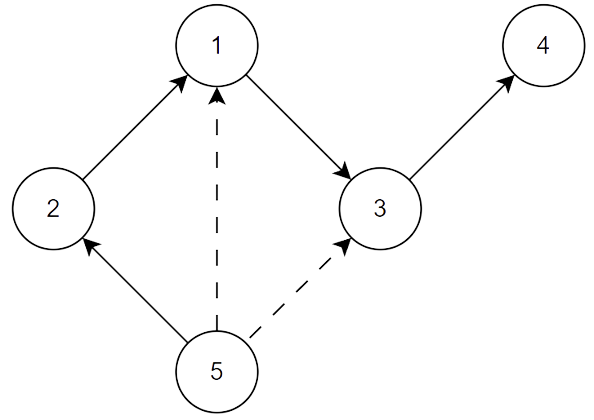
\includegraphics[width=0.5\linewidth]{images/conflictgraph.png}
        \end{figure}
        Some arcs can be omitted if the nodes are connected in another way (in this case we can remove arcs $\{\{5,1\},\{5,3\}\}$). 

        There are no cycles, so the schedule is CSR (and also VSR). 

    \newpage
    
    \section{Schedule classification}
        Classify the following schedule with respect to CSR and VSR classes:  
        \[r_2(u) w_2(s) r_1(x) r_2(y) w_3(y) r_5(x) w_5(u) w_3(s)w_2(u) w_3(x) w_1(u) r_4(y) w_5(z) r_5(z)\]
    \subsection*{Solution}
        Since CSR contains VSR we check with the conflict graph. To do so we first divide the schedule based on the resources: 
        \begin{itemize}
            \item $x: r_1 \: r_5 \:w_3$
            \item $y: r_2 \: w_3 \:r_4$
            \item $z: w_5 \: r_5$
            \item $s: w_2 \: w_3$
            \item $u: r_2 \: w_5 \: w_2 \:w_1$
        \end{itemize}
        The nodes are $\{1,2,3,4,5\}$ and the arcs are found with the write-write or write-read relations found in the previous groups. So we have the following graph:
        \begin{figure}[H]
            \centering
            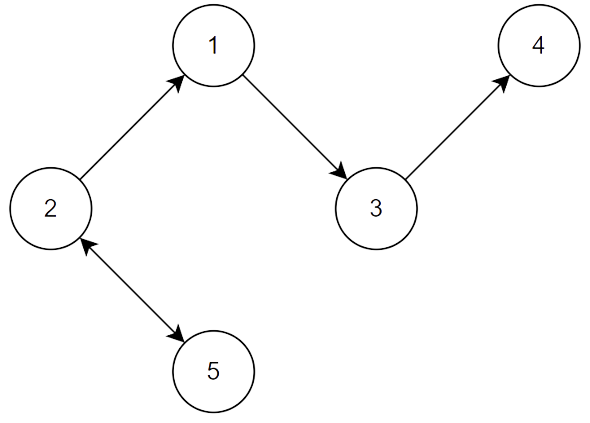
\includegraphics[width=0.5\linewidth]{images/conflictgraph1.png}
        \end{figure}
        It is possible to see that there is a cycle between two and five. The definition of VSR states that we need to have the same reads-from relations and final writes. So, we try to find a view-equivalent 
        schedule that is also CSR. One possible solution is simply to swap the two writes on the resource $u$ and that is sufficient to eliminate the cycle. So, the schedule: 
        \[r_2(u) w_2(s) r_1(x) r_2(y) w_3(y) r_5(x) w_5(u) w_2(u) w_3(s) w_3(x) w_1(u) r_4(y) w_5(z) r_5(z)\]
        is CSR and also VSR. 

    \newpage
    
    \section{Schedule classification}
        Classify the following schedule with respect to CSR and VSR classes:  
        \[r_1(x) r_2(y) w_3(y) r_5(x) w_5(u) w_3(s)w_2(u) w_3(x) w_1(u) r_4(y) w_5(z) r_5(z) r_2(u) w_2(s)\]
    \subsection*{Solution}
        Since CSR contains VSR we check with the conflict graph. To do so we first divide the schedule based on the resources: 
        \begin{itemize}
            \item $x: r_1 \: r_5 \: w_3$
            \item $y: r_2 \: w_3 \: r_4$
            \item $z: w_5 \: r_5$
            \item $s: w_3 \: w_2$
            \item $u: w_5 \: w_2 \: w_1 \: r_2$
        \end{itemize}
        The nodes are $\{1,2,3,4,5\}$ and the arcs are found with the write-write or write-read relations found in the previous groups. So we have the following graph:
        \begin{figure}[H]
            \centering
            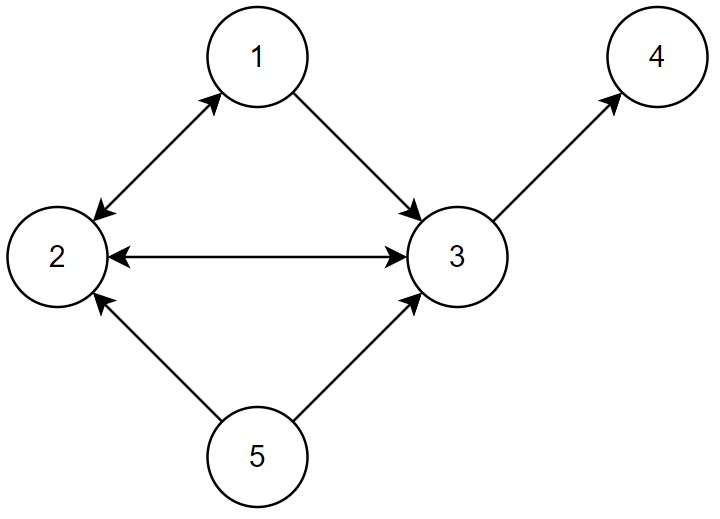
\includegraphics[width=0.5\linewidth]{images/conflictgraph2.png}
        \end{figure}
        In this case it is not possible to find a VSR schedule because it is impossible to do so without changing the final write on $s$. 

    \newpage

    \section{Schedule classification}
        Classify the following schedule with respect to CSR and VSR classes:  
        \[r_5(x) r_3(y) w_3(y) r_6(t) r_5(t) w_5(z) w_4(x) r_3(z) w_1(y) r_6(y) w_6(t) w_4(z) w_1(t) w_3(x) w_1(x) r_1(z) w_2(t) w_2(z)\]
    \subsection*{Solution}
        Since CSR contains VSR we check with the conflict graph. To do so we first divide the schedule based on the resources: 
        \begin{itemize}
            \item $t: \: r_6 \: r_5 \: w_6 \: w_1 \: w_2$
            \item $x: \: r_5 \: w_4 \: w_3 \: w_1$
            \item $y: \: r_3 \: w_3 \: w_1 \: r_6$
            \item $z: \: w_5 \: r_3 \: w_4 \: r_1 \: w_2$
        \end{itemize}
        The nodes are $\{1,2,3,4,5,6\}$ and the arcs are found with the write-write or write-read relations found in the previous groups. So we have the following graph:
        \begin{figure}[H]
            \centering
            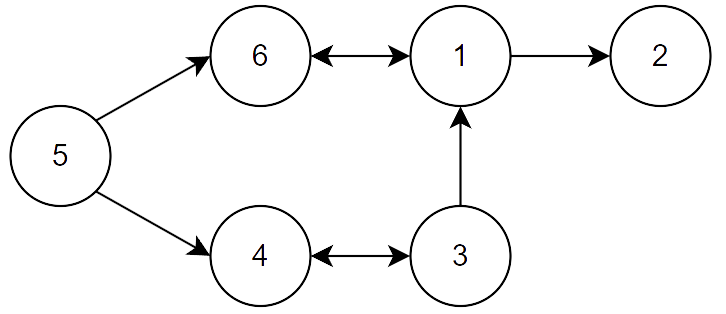
\includegraphics[width=0.5\linewidth]{images/conflictgraph3.png}
        \end{figure}
        We have two cycles. It is impossible to find a VSR schedule because only the conflict between four and three can be eliminated (the other one changes a read-write relation).

    \newpage

    \chapter{Exercise session II}
    \section{Schedule classification}
        Classify the following schedule with respect to 2PL and strict 2PL classes: 
        \[r_1(x) r_2(y) w_3(y) r_5(x) w_5(u) w_3(s) w_2(u) w_3(x) w_1(u) r_4(y) w_5(z) r_5(z)\]
    \subsection*{Solution}
        For strict 2PL we assume that all transactions commit and release all locks immediately after their last operation, and check if releases can be executed at commit time.
        \begin{table}[H]
            \centering
            \begin{tabular}{c|cccccccccccc}
                    & \textit{1} & \textit{2}      & \textit{3} & \textit{4} & \textit{5} & \textit{6} & \textit{7}                        & \textit{8}      & \textit{9}              & \textit{10} & \textit{11} & \textit{12}             \\ \hline
            \textit{S} &            &                 &            &            &            & $w_3$      &                                   &                 &                         &             &             &                         \\
            \textit{U} &            &                 &            &            & $w_5$      &            & $\searrow_5w_2\downharpoonleft_2$ &                 & $w_1\downharpoonleft_1$ &             &             &                         \\
            \textit{X} & $r_1$      &                 &            & $r_5$      &            &            &                                   & $\searrow_1w_3$ &                         &             &             &                         \\
            \textit{Y} &            & $r_2\searrow_2$ & $w_3$      &            &            &            &                                   &                 &                         & $r_4$       &             &                         \\
            \textit{Z} &            &                 &            &            &            &            &                                   &                 &                         &             & $w_5$       & $r_5\downharpoonleft_5$
            \end{tabular}
        \end{table}
        $S$ clearly cannot be in strict 2PL. The contradictions are:
        \begin{itemize}
            \item $T_1$ must release $X$ before $8$. 
            \item $T_2$ must release $Y$ before $7$.
            \item $T_5$ must release $U$ before $12$.
        \end{itemize}
        For 2PL we have:
        \begin{table}[H]
            \centering
            \resizebox{\columnwidth}{!}{%
            \begin{tabular}{c|cccccccccccc}
                    & \textit{1} & \textit{2}      & \textit{3} & \textit{4} & \textit{5} & \textit{6} & \textit{7}                        & \textit{8}      & \textit{9}              & \textit{10} & \textit{11} & \textit{12}             \\ \hline
            \textit{S} &                            &                                   &                           &                           &                           & $\nearrow_3w_3$       &                                       & $\searrow_3$                          &                         &                             &             &                         \\
            \textit{U} &                            &                                   &                           &                           & $\nearrow_5w_5\searrow_5$ &                       & $\nearrow_2w_2\searrow_2\nearrow_1$   &                                       & $w_1\searrow_1$         &                             &             &                         \\
            \textit{X} & $\nearrow_1r_1$            &                                   &                           & $\nearrow_5r_5$           &                           & $\searrow_5$          &                                       & $\searrow_1\nearrow_3w_3\searrow_3$   &                         &                             &             &                         \\
            \textit{Y} &                            & $\nearrow_2r_2\searrow_2$         & $\nearrow_3w_3$           &                           &                           &                       &                                       &                                       & $\searrow_3$            & $\nearrow_4r_4\searrow_4$   &             &                         \\
            \textit{Z} &                            &                                   &                           & $\nearrow_5$              &                           &                       &                                       &                                       &                         &                             & $w_5$       & $r_5\searrow_5$
            \end{tabular}%
            }
        \end{table}
        It is also not in 2PL: an assignment is not possible for $T_2$ (which must release $Y$ before locking $U$).

    \newpage

    \section{Schedule classification}
        Classify the following schedule with respect to 2PL and strict 2PL classes: 
        \[r_4(x) r_2(x) w_4(x) w_2(y) w_4(y) r_3(y) w_3(x) w_4(z) r_3(z) r_6(z) r_8(z) w_6(z) w_9(z) r_5(z) r_10(z)\]
    \subsection*{Solution}
        For strict 2PL we assume that all transactions commit and release all locks immediately after their last operation, and check if releases can be executed at commit time.
        \begin{table}[H]
            \centering
            \begin{tabular}{c|ccccccccccccccc}
                       & \textit{1} & \textit{2} & \textit{3} & \textit{4} & \textit{5} & \textit{6} & \textit{7} & \textit{8} & \textit{9} & \textit{10} & \textit{11} & \textit{12} & \textit{13} & \textit{14} & \textit{15} \\ \hline
            \textit{X} & $r_4$      & $r_2\searrow _2$          & $w_4$      &                              &            &            & $w_3$      &            &            &             &             &             &             &             &             \\
            \textit{Y} &            &                           &            & $w_2\downharpoonleft_2$      & $w_4$      & $r_3$      &            &            &            &             &             &             &             &             &             \\
            \textit{Z} &            &                           &            &                              &            &            &            & $w_4$      & $r_3$      & $r_6$       & $r_8$       & $w_6$       & $w_9$       & $r_5$       & $r_{10}$     
            \end{tabular}%
        \end{table}
        It is therefore clear that the schedule cannot be in 2PL-strict, due to $T_2$ and $T_4$: $T_2$ ends after 4, but $T_4$ wants to write $X$ at 3, and $T_2$ would thus be 
        required to release $X$ earlier, which is impossible if $T_2$ has to keep all locks until after 4.

        For 2PL we have:
        \begin{table}[H]
            \centering
            \resizebox{\columnwidth}{!}{%
            \begin{tabular}{c|ccccccccccccccc}
                       & \textit{1} & \textit{2} & \textit{3} & \textit{4} & \textit{5} & \textit{6} & \textit{7} & \textit{8} & \textit{9} & \textit{10} & \textit{11} & \textit{12} & \textit{13} & \textit{14} & \textit{15} \\ \hline
            \textit{X} & $\nearrow_4r_4$        & $\nearrow_2r_2\searrow_2$         & $\nearrow_4w_4$       &                       & $\searrow_4$                          &                           & $\nearrow_3w_3$       &                       &                          & $\searrow_3$  &                       &             &             &             &             \\
            \textit{Y} &                        & $\nearrow_2$                      &                       & $w_2\searrow_2$       & $\nearrow_4w_4\searrow_4$             & $\nearrow_3r_3$           &                       &                       &                          & $\searrow_3$  &                       &             &             &             &             \\
            \textit{Z} &                        &                                   & $\nearrow_4$          &                       &                                       &                           &                       & $w_4\searrow_4$       & $\nearrow_3r_3$          & $r_6$         & $r_8\searrow_3$       & $w_6$       & $w_9$       & $r_5$       & $r_{10}$     
            \end{tabular}%
            }
        \end{table}
        We need to look at those acquisitions that must be anticipated and to those releases that must be delayed to not violate the 2PL rules.
        $T_4$ can only get the XL on X only after 2 and on $Y$ after 4 and has to release $Y$ before 6 and $X$ before 7. Thus, the lock on $Z$ must be acquired before 6.
        $T_2$ can get all the locks at the beginning and release them immediately after each use. $T_3$ can acquire $X$, $Y$ and $Z$ just before using them and release them all before 12. 
        All other transactions ($T_6, T_9, T_5, T_{10}$) clearly pose no problems.

    \newpage

    \section{Schedule classification}
        Classify the following schedule with respect to 2PL and strict 2PL classes: 
        \[r_1(A) r_2(A) w_2(A) r_1(B) w_1(C) w_2(C) r_3(C) w_3(A) w_2(B) w_3(B)\]
    \subsection*{Solution}
        For strict 2PL we assume that all transactions commit and release all locks immediately after their last operation, and check if releases can be executed at commit time.
        \begin{table}[H]
            \centering
            \begin{tabular}{c|cccccccccc}
                    & \textit{1} & \textit{2} & \textit{3} & \textit{4} & \textit{5} & \textit{6} & \textit{7} & \textit{8} & \textit{9} & \textit{10} \\ \hline
            \textit{A} & $r_1$      & $r_2\searrow _1$          & $w_2$      &            &            &            &            & $w_3$      &            &             \\
            \textit{B} &            &                           &            &            & $w_1\downharpoonleft_1$      & $w_2$      & $r_3$      &            &            &             \\
            \textit{C} &            &                           &            & $r_1$      &            &            &            &            & $w_2$      & $w_3$      
            \end{tabular}%
        \end{table}
        The schedule is not strict 2PL.

        For 2PL we have:
        \begin{table}[H]
            \centering
            \resizebox{\columnwidth}{!}{%
            \begin{tabular}{c|cccccccccc}
                    & \textit{1} & \textit{2} & \textit{3} & \textit{4} & \textit{5} & \textit{6} & \textit{7} & \textit{8} & \textit{9} & \textit{10} \\ \hline
            \textit{A} & $\nearrow_1r_1$        & $\nearrow_2r_2\searrow_1$         & $\nearrow_2w_2$       &                   &                   & $\searrow_2$                      &                           & $\nearrow_3w_3$       &                       & $\searrow_3$            \\
            \textit{B} &                        & $\nearrow_1$                      &                       &                   & $w_1\searrow_1$   & $\nearrow_2w_2\searrow_2$         & $\nearrow_3r_3$           &                       &                       & $\searrow_3$            \\
            \textit{C} &                        & $\nearrow_1$                      &                       & $r_1\searrow_1$   &                   &                                   &                           &                       & $w_2\searrow_2$       & $\nearrow_3w_3\searrow_3$      
            \end{tabular}%
            }
        \end{table}
        The schedule is 2PL. 

    \newpage

    \section{Schedule classification}
        Classify the following schedule with respect to 2PL and strict 2PL classes: 
        \[r_1(x) w_2(x) r_1(z) w_1(y) r_3(x) r_4(x) w_3(z) w_2(y) r_3(y) w_4(x) w_4(y)\]
    \subsection*{Solution}
        For strict 2PL we assume that all transactions commit and release all locks immediately after their last operation, and check if releases can be executed at commit time.
        \begin{table}[H]
            \centering
            \begin{tabular}{c|ccccccccccc}
                       & \textit{1} & \textit{2} & \textit{3} & \textit{4} & \textit{5} & \textit{6} & \textit{7} & \textit{8} & \textit{9} & \textit{10} & \textit{11}          \\ \hline
            \textit{X} & $r_1\searrow_1$       & $w_2$      &            &                                  & $r_3$      & $r_4$      &            &            &            & $w_4$       &                    \\
            \textit{Y} &                       &            &            & $w_1\downharpoonleft_1$          &            &            &            & $w_2$      & $r_3$      &             & $w_4$                \\
            \textit{Z} &                       &            & $r_1$      &                                  &            &            & $w_3$      &            &            &             &                     
            \end{tabular}%
        \end{table}
        The schedule is not strict 2PL.

        For 2PL we have:
        \begin{table}[H]
            \centering
            \resizebox{\columnwidth}{!}{%
            \begin{tabular}{c|ccccccccccc}
                       & \textit{1} & \textit{2} & \textit{3} & \textit{4} & \textit{5} & \textit{6} & \textit{7} & \textit{8} & \textit{9} & \textit{10} & \textit{11}          \\ \hline
            \textit{X} & $\nearrow_1r_1\searrow_1$              & $\nearrow_2w_2$       &                       &                                   & $\searrow_2\nearrow_3r_3$         & $\nearrow_4r_4$       &                       &                   & $\searrow_3$                   & $\nearrow_4w_4$       & $\searrow_4$     \\
            \textit{Y} & $\nearrow_1$                           &                       &                       & $w_1\searrow_1\nearrow_2$         &                                   &                       &                       & $w_2\searrow_2$   & $\nearrow_3r_3\searrow_3$      &                       & $\nearrow_4w_4\searrow_4$                \\
            \textit{Z} & $\nearrow_1$                           &                       & $r_1\searrow_1$       &                                   &                                   &                       & $\nearrow_3w_3$       &                   & $\searrow_3$                   &                       &                     
            \end{tabular}%
            }
        \end{table}
        The schedule is 2PL. 

    \newpage

    \section{Update locks}
        Given the schedule:
        \[r1(x) r2(x) r3(y) w3(y) w1(x) w2(y)\]
        show the sequence of lock and unlock requests produced by the transactions in a 2PL execution, in a system with update lock (available locks: $SL, UL, XL$).
    \subsection*{Solution}
        The locking phases with update locks are the following: 
        \begin{table}[H]
            \centering
            \begin{tabular}{|c|c|}
            \hline
            $X$                                           & $Y$                                           \\ \hline
            $\textnormal{UL}_1(x)$                        &                                               \\
            $r_1(x)$                                      &                                               \\
            $\textnormal{SL}_2(x)$                        &                                               \\
            $r_2(x)$                                      &                                               \\
                                                          & $\textnormal{UL}_3(y)$                        \\
                                                          & $r_3(y)$                                      \\
                                                          & $\textnormal{XL}_3(y) [\textnormal{upgrade}]$ \\
                                                          & $w_3(y)$                                      \\
                                                          & $\textnormal{rel}(\textnormal{XL}_3(y))$      \\
                                                          & $\textnormal{XL}_2(y)$                        \\
            $\textnormal{rel}(\textnormal{SL}_2(x))$      &                                               \\
            $\textnormal{XL}_1(x) [\textnormal{upgrade}]$ &                                               \\
            $w_1(x)$                                      &                                               \\
            $\textnormal{rel}(\textnormal{XL}_1(x))$      &                                               \\
                                                          & $w_2(y)$                                      \\
                                                          & $\textnormal{rel}(\textnormal{XL}_2(y))$      \\ \hline
            \end{tabular}
        \end{table}

    \newpage

    \section{Update locks}
        Update lock was introduced to contrast deadlocks. Can we state that deadlocks are impossible in the presence of update locks?
        \begin{enumerate}
            \item If so, concisely explain why. 
            \item If not, provide a counter-example.
        \end{enumerate}
    \subsection*{Solution}
        \begin{enumerate}
            \item Clearly deadlocks are possible in the presence of UL. Indeed, UL only makes deadlock less likely, by preventing one type of deadlock, due to 
                update patterns, when two transactions compete for the same resource ($r_1(x) r_2(x) w_1(x) w_2(x)$). 
            \item Consider two distinct resources $X$ and $Y$, and two transactions that want to access them in this order: $r_1(X) r_2(Y) w_1(Y) w_2(X)$. It is likely that they end up 
                in deadlock, especially if the system on which they run applies 2PL. UL is totally irrelevant here, because there is no update pattern. 
        \end{enumerate}

\newpage

\chapter{Exercise session III}
    \section{Obermarck's algorithm}
        Consider the following waiting conditions:
        \begin{itemize}
            \item Node $A$: $E_B \rightarrow t_1, t_1 \rightarrow t_2, E_C \rightarrow t_2, t_2 \rightarrow t_3, t_3 \rightarrow E_B, E_B \rightarrow t_4, t_4 \rightarrow t_3$
            \item Node $B$: $E_A \rightarrow t_3, t_3 \rightarrow t_5, t_5 \rightarrow t_6, t_6 \rightarrow E_C, E_C \rightarrow t_7, t_7 \rightarrow t_6, t_9 \rightarrow t_4,t_4 \rightarrow E_A, t_1 \rightarrow E_A$
            \item Node $C$: $E_B \rightarrow t_6, t_6 \rightarrow t_8, t_8 \rightarrow t_2, t_2 \rightarrow E_A, t_7 \rightarrow E_B$
        \end{itemize}
        Simulate the Obermarck algorithm and indicate whether there is a distributed deadlock.
    \subsection*{Solution}
        We need to construct the graph with the given constraints, that is: 
        \begin{figure}[H]
            \centering
            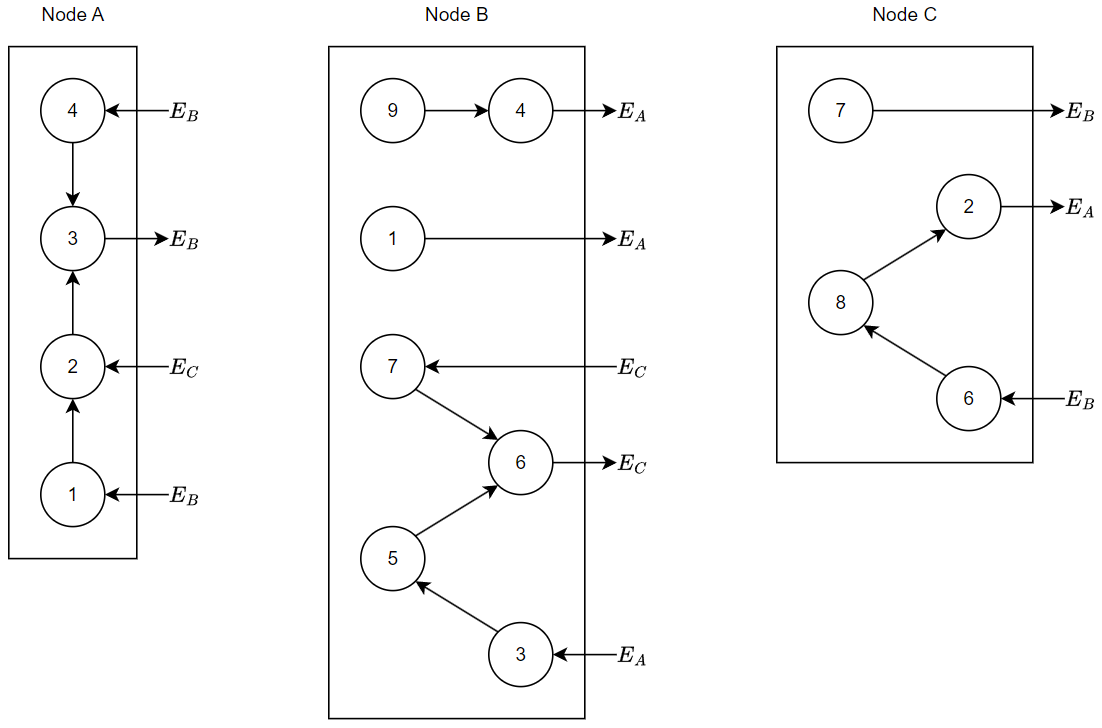
\includegraphics[width=0.6\linewidth]{images/Ob1.png}
        \end{figure}
        We have to check all the nodes where the sender has a lower value than the receiver. In this case we have that the update is sent to the 
        other distributed node. The interesting cases are highlighted in the image. So, we now have to add the nodes: 
        \begin{itemize}
            \item $4 \rightarrow 3$ in $E_B$. 
            \item $7 \rightarrow 6$ in $E_C$. 
            \item $6 \rightarrow 2$ in $E_A$. 
        \end{itemize}
        If the numbered node is not present we can add it to the graph of the distributed node. We obtain the following graphs: 
        \begin{figure}[H]
            \centering
            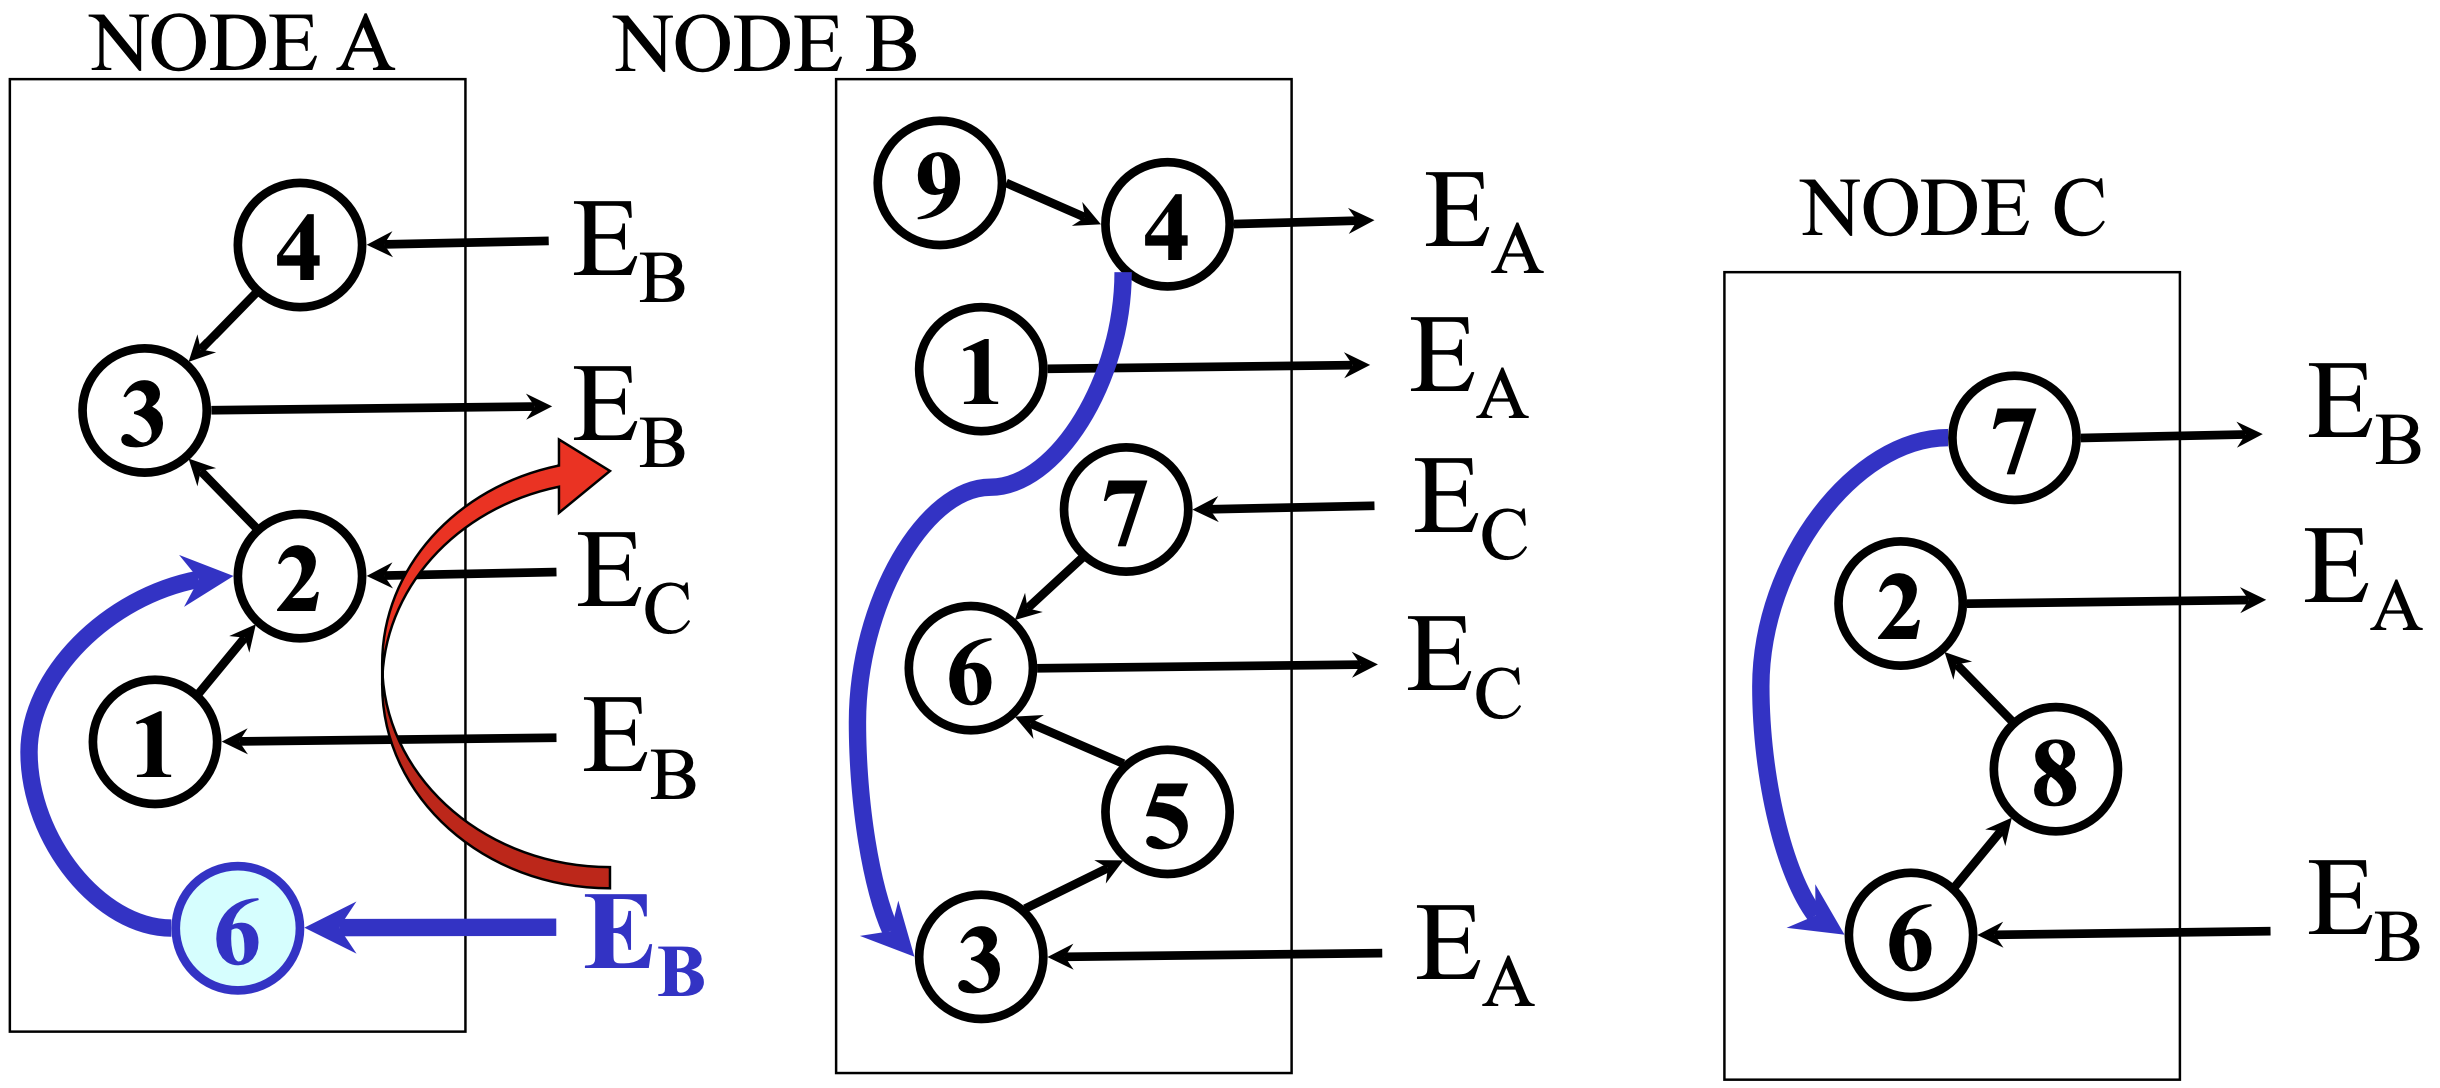
\includegraphics[width=0.6\linewidth]{images/Ob2.png}
        \end{figure}
        We have to check if other messages are sent. We have:
        \begin{itemize}
            \item $6 \rightarrow 3$ in $E_B$. 
        \end{itemize}
        So the updated graph is: 
        \begin{figure}[H]
            \centering
            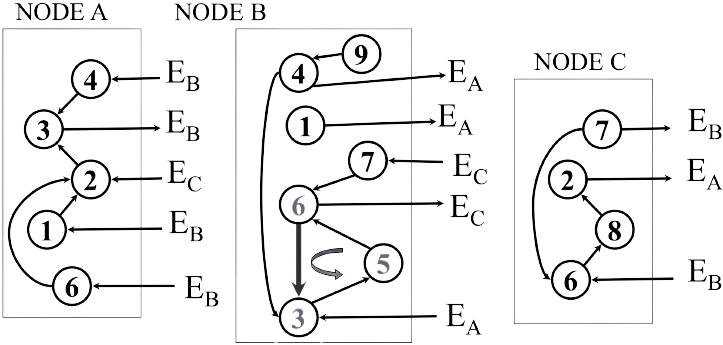
\includegraphics[width=0.6\linewidth]{images/Ob3.png}
        \end{figure}
        We have found a cycle, so there is a deadlock. 

    \newpage

    \section{Obermarck's algorithm}
        The nodes $A$, $B$, and $C$ of a distributed transactional system are aware of the following remote and local waiting conditions:
        \begin{itemize}
            \item Node $A: E_B \rightarrow t_3, E_C \rightarrow t_2, t_1 \rightarrow E_C, t_3 \rightarrow t_5, t_5 \rightarrow t_1$
            \item Node $B: E_C \rightarrow t_2, t_3 \rightarrow E_A, t_2 \rightarrow t_3$
            \item Node $C: t_2 \rightarrow E_A, t_2 \rightarrow E_B, t_1 \rightarrow t_4, t_4 \rightarrow t_2$
        \end{itemize}
        Execute the Obermarck's algorithm twice, with different conventions:
        \begin{enumerate}
            \item Sending messages of the form $E_X \rightarrow t_i \rightarrow t_j \rightarrow E_Y$ forward (toward node $Y$) and only 
                if and only if $i > j$. 
            \item With the opposite conventions, so if and only if $i > j$
        \end{enumerate}
        Discuss the outcome, and explain it, taking into account the properties of the algorithm and the initial conditions.
    \subsection*{Solution}
        The graph is the following: 
        \begin{figure}[H]
            \centering
            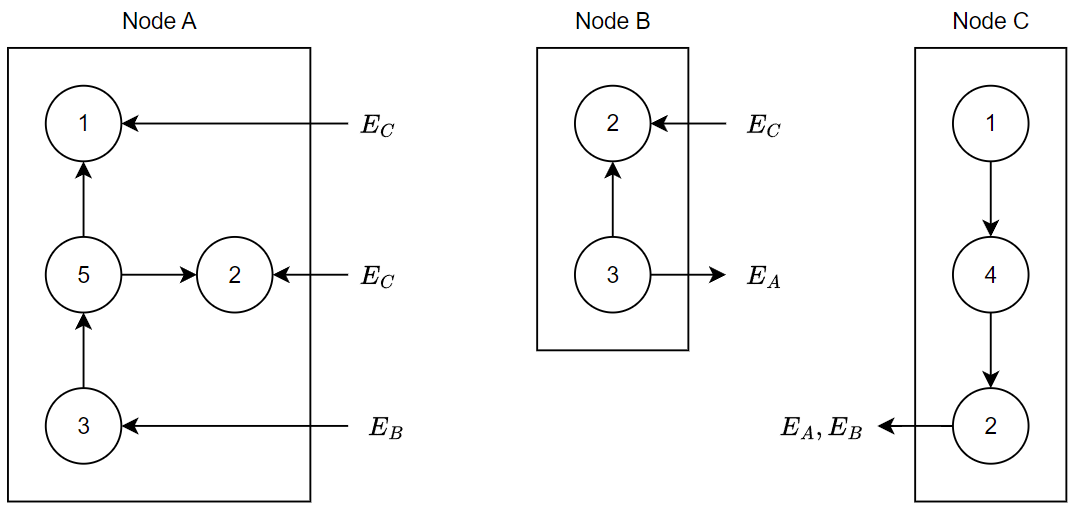
\includegraphics[width=0.6\linewidth]{images/Ob4.png}
        \end{figure}
        \begin{enumerate}
            \item We have to add the nodes (connections are distributed): 
                \begin{itemize}
                    \item $3 \rightarrow 1$ in $E_C$. 
                    \item $3 \rightarrow 2$ in $E_A$. 
                    \item $3 \rightarrow 2$ in $E_B$. 
                \end{itemize}
                By adding those nodes we found that the third one creates a deadlock. 
            \item We have to add the node (connections are distributed): 
                \begin{itemize}
                    \item $2 \rightarrow 3$ in $E_A$. 
                \end{itemize}
                No cycles are found, so no deadlocks found. 
        \end{enumerate}
        The algorithm is independent of the conventions but the initial conventions, but the initial conditions must be consistent and complete. 
        On a faulty dataset even the best algorithm returns untrustworthy results. In this case we have a link missing between node $A$ and $C$.

    \newpage

    \section{Schedule classification}
        Classify the following schedule with respect to timestamps: 
        \[r_4(x) r_2(x) w_4(x) w_2(y) w_4(y) r_3(y) w_3(x) w_4(z) r_3(z) r_6(z) r_8(z) w_6(z) w_9(z) r_5(z) r_{10}(z)\]
    \subsection*{Solution}
        We can identify pairs of operations that cause killings:
        \begin{itemize}
            \item $X: r_4 r_2 w_4 w_3$
            \item $Y: w_2 w_4 r_3$
            \item $Z: w_4 r_3 r_6 r_8 w_6 w_9 r_5 r_{10}$
        \end{itemize}
        On $X$ we have that $w_3$ is too late with respect to $r_4$ and $w_4$. On $Y$ we have that $r_3$ is late with respect to $w_4$. On 
        $Z$ we have that $r_3$ is late with respect to $w_4$, $w_6$ with respect to $r_8$, $r_5$ with respect to both $w_6$ and $w_9$. 
        So, the schedule is not in TS-mono. 

        The schedule is also outside TS-multi, because $w_3(X)$ comes too late ($r_4(X)$ was already given the initial version instead) and 
        also because $w_6(Z)$ is late with respect to $r_8(Z)$. The other five reasons were due to reads (that are always accepted in TS-multi).

    \newpage

    \section{Schedule classification}
        Classify the following schedule with respect to timestamps: 
        \[r_1(x) r_2(y) w_3(y) r_5(x) w_5(u) w_3(s) w_2(u) w_3(x) w_1(u) r_4(y) w_5(z) r_5(z)\]
    \subsection*{Solution}
        We can identify pairs of operations that cause killings:
        \begin{itemize}
            \item $S:w_3$
            \item $U:w_5w_2w_1$
            \item $X:r_1r_5w_3$
            \item $Y:r_2w_3r_4$
            \item $Z:w_5r_5$
        \end{itemize}
        $S$, $Y$ and $Z$ are ok, $U$ is ok only if the Thomas rule is applied, and $X$ is not ok for both TS-mono and TS-multi. 


    \newpage

    \section{Schedule classification}
        Classify the following schedule:
        \[r_1(X) w_1(Y) w_2(Y) w_3(Z) r_1(Z) w_4(X) r_4(Y) w_3(X) r_5(Y) w_5(X)\] 
    \subsection*{Solution}
        First, we check if it is CSR:
        \begin{itemize}
            \item $X: r_1 w_4 w_3 w_5$
            \item $Y: w_1 w_2 r_4 r_5$
            \item $Z: w_3 r_1$
        \end{itemize}
        We found a cycle between the nodes three and one, so it is not CSR. It is also not VSR. We now check for TS using the same list: 
        we find that $w_4 w_3$ are not in the correct order, so it is not in TS-mono, neither in TS-multi (it is a write that causes the 
        problem).

    \newpage

    \section{Schedule classification}
        Classify the following schedule:
        \[r_1(x) r_2(y) w_3(x) r_5(z) w_6(z) w_2(x) w_3(y) r_7(z) w_4(x)\] 
    \subsection*{Solution}
        First, we check if it is CSR:
        \begin{itemize}
            \item $X: r_1 w_3 w_2 w_4$
            \item $Y: r_2 w_3$
            \item $Z: r_5 w_6 r_7$
        \end{itemize}
        There is a cycle between two and three, so it is not CSR, but by swapping $w_3 w_2$ we can obtain a VSR schedule without changing the 
        schedule. 

        The schedule is not TS-mono because we have $w_3 w_2$ and so also non TS-multi. 
   
    \newpage 

    \section{Schedule classification}
        Given the resources above and the following transactions:
        \[T_1: r_1(C) w_1(B) w_1(C)\] 
        \[T_2: w_2(A) r_2(C)\]
        Consider that $T_1$ and $T_2$ can only be scheduled in 10 different ways (two serial, eight interleaved). What can be stated about 
        the 2PL-strict compatibility of these schedules? 
    \subsection*{Solution}
        We note that the only potential conflict is between $w_1(C)$ and $r_2(C)$. But these are also the last operations of their respective 
        transactions: to check for compatibility, we can always assume that the commit occurs right after the last operation, and that all 
        locks are released in favor of the other one. But this argument is independent of the order of the operations, and is therefore valid 
        for all the eight interleaved schedules. So, all the schedules are strict 2PL. 

    \newpage

    \section{Hierarchical lock}
        \begin{figure}[H]
            \centering
            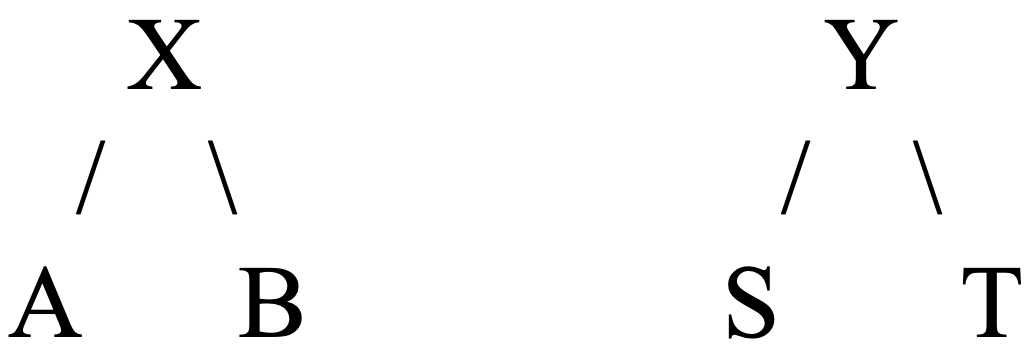
\includegraphics[width=0.4\linewidth]{images/HL1.png}
        \end{figure}
        Given the resource hierarchy above, is the following schedule compatible with a 2PL-strict scheduler that applies hierarchical locking?
        \[r_1(A) w_1(S) w_2(T) r_2(A) w_1(A)\]
    \subsection*{Solution}
        The lock manager works as follows: 
        \begin{table}[H]
            \centering
            \begin{tabular}{c|cccccc|c}
            \cline{2-7}
            \textit{}                          & \textit{X}               & \textit{A}              & \textit{B} & \textit{Y}               & \textit{S}          & \textit{T}          & \textit{}    \\ \cline{1-7}
            \multicolumn{1}{|c|}{$r_1(A)$}     & $\textnormal{ISL}_1$     & -                       & -          & -                        & -                   & -                   &              \\
            \multicolumn{1}{|c|}{}             & $\textnormal{ISL}_1$     & $\textnormal{SL}_1$     & -          & -                        & -                   & -                   &              \\
            \multicolumn{1}{|c|}{$w_1(S)$}     & $\textnormal{ISL}_1$     & $\textnormal{SL}_1$     & -          & $\textnormal{IXL}_1$     & -                   & -                   &              \\
            \multicolumn{1}{|c|}{}             & $\textnormal{ISL}_1$     & $\textnormal{SL}_1$     & -          & $\textnormal{IXL}_1$     & $\textnormal{XL}_1$ & -                   &              \\
            \multicolumn{1}{|c|}{$w_2(T)$}     & $\textnormal{ISL}_1$     & $\textnormal{SL}_1$     & -          & $\textnormal{IXL}_{1,2}$ & $\textnormal{XL}_1$ & -                   &              \\
            \multicolumn{1}{|c|}{}             & $\textnormal{ISL}_1$     & $\textnormal{SL}_1$     & -          & $\textnormal{IXL}_{1,2}$ & $\textnormal{XL}_1$ & $\textnormal{XL}_2$ &              \\
            \multicolumn{1}{|c|}{$r_2(A)$}     & $\textnormal{ISL}_{1,2}$ & $\textnormal{SL}_1$     & -          & $\textnormal{IXL}_{1,2}$ & $\textnormal{XL}_1$ & $\textnormal{XL}_2$ &              \\
            \multicolumn{1}{|c|}{}             & $\textnormal{ISL}_{1,2}$ & $\textnormal{SL}_{1,2}$ & -          & $\textnormal{IXL}_{1,2}$ & $\textnormal{XL}_1$ & $\textnormal{XL}_2$ &              \\
            \multicolumn{1}{|c|}{commit $T_2$} &                          &                         &            &                          &                     &                     & End of $T_2$ \\
            \multicolumn{1}{|c|}{}             & $\textbf{ISL}_1$         & $\textnormal{SL}_1$     & -          & $\textnormal{IXL}_1$     & $\textnormal{XL}_1$ & -                   &              \\
            \multicolumn{1}{|c|}{$w_1(A)$}     & $\textbf{IXL}_1$         & $\textbf{SL}_1$         & -          & $\textnormal{IXL}_1$     & $\textnormal{XL}_1$ & -                   &              \\
            \multicolumn{1}{|c|}{}             & $\textnormal{IXL}_1$     & $\textbf{XL}_1$         & -          & $\textnormal{IXL}_1$     & $\textnormal{XL}_1$ & -                   &              \\
            \multicolumn{1}{|c|}{commit $T_1$} &                          &                         &            &                          &                     &                     & End of $T_1$ \\ \cline{1-7}
            \end{tabular}
        \end{table}
        So, it is compatible with a strict 2PL scheduler. 

    \newpage

    \section{Hierarchical lock}
        Consider the following short schedule occurring on a system with hierarchical lock over a hierarchy where $PagA$ contains tuples 
        $t_1$ and $t_2$:
        \[r_1( PagA ), w_2( t1 ), w_1( t2 )\]
        Show a possible sequence of locks, unlocks, lock upgrades, and lock downgrades performed by transactions $T_1$ and $T_2$ such that
        the schedule is in 2PL.
    \subsection*{Solution}
        We have that: 
        \begin{table}[H]
            \centering
            \begin{tabular}{c|ccc|}
            \cline{2-4}
            \textit{}                    & \textbf{PagA}                           & \textbf{t2}          & \textbf{t1}           \\ \cline{2-4} 
            $\textnormal{SIXL}_1(PagA)$  & $\textnormal{SIXL}_1$                   & -                    & -                     \\
            $\textnormal{XL}_1(t2)$      & $\textnormal{SIXL}_1$                   & $\textnormal{XL}_1$  & -                     \\
            $r_1(PagA)$                  &                                         &                      &                       \\
            $\textnormal{U-SL}_1(PagA)$  & $\textnormal{IXL}_1,\textnormal{IXL}_2$ & $\textnormal{XL}_1$  & -                     \\
            $\textnormal{IXL}_2(PagA)$   & $\textnormal{IXL}_1,\textnormal{IXL}_2$ & $\textnormal{XL}_1$  & -                     \\
            $\textnormal{XL}_2(t1)$      & $\textnormal{IXL}_1,\textnormal{IXL}_2$ & $\textnormal{XL}_1$  & $\textnormal{XL}_2$   \\
            $w_2(t1)$                    &                                         &                      &                       \\
            $\textnormal{U-XL}_2(t1)$    & $\textnormal{IXL}_1,\textnormal{IXL}_2$ & $\textnormal{XL}_1$  & -                     \\
            $\textnormal{U-IXL}_2(PagA)$ & $\textnormal{IXL}_1$                    & $\textnormal{XL}_1$  & -                     \\
            Commit $T_2$                 &                                         &                      &                       \\
            $w_1(t2)$                    &                                         &                      &                       \\
            $\textnormal{U-XL}_1(t2)$    & $\textnormal{IXL}_1$                    & -                    & -                     \\
            $\textnormal{U-IXL}_1(PagA)$ & -                                       & -                    & -                     \\
            Commit $T_1$                 & \multicolumn{1}{l}{}                    & \multicolumn{1}{l}{} & \multicolumn{1}{l|}{} \\ \cline{2-4} 
            \end{tabular}
        \end{table}
        So the schedule is 2PL.

    \newpage 

    \chapter{Exercise session IV}
    \section{Ranking and skyline queries}
        Consider a distributed setting with three data sources, ranking basketball players according to their offensive rating (off), defensive rating (def) and rebounds (reb).
        An associated score in $[0,1]$ is indicated (the higher, the better). Sorted access is available.
        \begin{table}[H]
            \centering
            \begin{tabular}{|cc|cc|cc|}
            \hline
            $\boldsymbol{R_0}$ \textbf{(off)} & \textbf{Player} & $\boldsymbol{R_1}$ \textbf{(def)} & \textbf{Player} & $\boldsymbol{R_2}$ \textbf{(reb)} & \textbf{Player} \\ \hline
            0.8         & 9      & 0.9         & 4      & 0.6         & 1      \\
            0.8         & 8      & 0.8         & 5      & 0.5         & 3      \\
            0.8         & 2      & 0.7         & 7      & 0.3         & 4      \\
            0.7         & 7      & 0.6         & 9      & 0.3         & 2      \\
            0.6         & 3      & 0.5         & 0      & 0.3         & 0      \\
            0.6         & 1      & 0.4         & 6      & 0.2         & 8      \\
            0.5         & 6      & 0.2         & 3      & 0.2         & 6      \\
            0.5         & 5      & 0.2         & 2      & 0.1         & 5      \\
            0.5         & 0      & 0.0         & 8      & 0.0         & 9      \\
            0.2         & 4      & 0.0         & 1      & 0.0         & 7      \\ \hline
            \end{tabular}
        \end{table}
        \begin{enumerate}
            \item Determine the top-3 players according to their median rank using MedRank.
            \item Remove the first data source and consider the scoring function
                \[\textnormal{MAX}(o) = \max\{\textnormal{def}(o), \textnormal{reb}(o)\}\] 
                Determine the top-2 players according to MAX using the algorithms $B_0$ and NRA.
            \item Assume now that random access is also available. Determine the top-2 players according to MAX with the algorithms TA and FA.
            \item Consider now the scoring function 
                \[\textnormal{SUM}(o) = \textnormal{def}(o) + \textnormal{reb}(o)\] 
                equally weighing all partial scores. What are the top-2 players according to SUM?
            \item Assume now that all the data regarding the players are centralized in a single data source, in which the players are available sortedly according to SUM. 
                Use SFS to determine the skyline of the players.
            \item Identify the players in the 2-skyband, and in the 3-skyband.
        \end{enumerate}
    \subsection*{Solution}
    \begin{enumerate}
        \item A player is considered when, while doing sorted access it appears in at least two tables. If we check the first row we find the following players: 
            $\{9,4,1\}$ and the tables are three, so no player appears in at least two tables. For the second iteration we have found $\{9,4,1,8,5,3\}$, so again
            no duplicate player. With the third row we have $\{9,4,1,8,5,3,2,7,4\}$. We have found the first player that appears in at least two rankings, but we 
            need two more players, so we can check the fourth row: $\{9,4,1,8,5,3,2,7,4,7,9,2\}$. With this iteration we have found other three players, and 
            the algorithm stops. The content of the buffer at this step is the following: 
            \begin{table}[H]
                \centering
                \begin{tabular}{|c|ccc|}
                \hline
                \textbf{Player} & \textbf{First row} & \textbf{Second row} & \textbf{Third row} \\ \hline
                4               & 1                  & 3                   & ?                  \\
                2               & 3                  & 4                   & ?                  \\
                7               & 3                  & 4                   & ?                  \\ 
                9               & 1                  & 4                   & ?                  \\
                1               & 1                  & ?                   & ?                  \\
                8               & 2                  & ?                   & ?                  \\
                5               & 2                  & ?                   & ?                  \\
                3               & 2                  & ?                   & ?                  \\ \hline
                \end{tabular}
            \end{table}
            With this algorithm we have found that the best players are: nine, four, two, and seven. In particular, the player four is the best 
            due to the median rank and the other three are equally good. 
        \item Since we have $k=2$, for the $B_0$ algorithm we need to make two sorted access to the first two rows, and add the objects to the buffer: 
            \begin{table}[H]
                \centering
                \begin{tabular}{c|cc|c}
                \hline
                \textbf{Player} & \textbf{$\boldsymbol{R_1}$ (def)} & \textbf{$\boldsymbol{R_2}$ (reb)} & \textbf{MAX} \\ \hline
                4               & 0.9                               & ?                                 & 0.9                             \\
                5               & 0.8                               & ?                                 & 0.8                             \\
                1               & ?                                 & 0.6                               & 0.6                             \\
                3               & ?                                 & 0.6                               & 0.6                             \\ \hline
                \end{tabular}
            \end{table}
            For each object in the buffer we have to make some random accesses to find the missing values. The buffer will be updated like follows. 
            \begin{table}[H]
                \centering
                \begin{tabular}{c|cc|c}
                \hline
                \textbf{Player} & \textbf{$\boldsymbol{R_1}$ (def)} & \textbf{$\boldsymbol{R_2}$ (reb)} & \textbf{MAX} \\ \hline
                4               & 0.9                               & 0.3                               & 0.9                             \\
                5               & 0.8                               & 0.1                               & 0.8                             \\
                1               & 0.0                               & 0.6                               & 0.6                             \\
                3               & 0.2                               & 0.6                               & 0.6                             \\ \hline
                \end{tabular}
            \end{table}
            The best two players in the buffer are four and five.

            For the NRA algorithm we have to make a sorted access to each row until the upper bound of the first element out of the top-$k$ is less
            or equal than the lower bound of the worst top-$k$. With the sorted access to the first row we have the following buffer. 
            \begin{table}[H]
                \centering
                \begin{tabular}{c|cc|cc}
                \hline
                \textbf{Player} & \textbf{$\boldsymbol{R_1}$ (def)} & \textbf{$\boldsymbol{R_2}$ (reb)} & \textbf{Lower bound} & \textbf{Upper bound} \\ \hline
                4               & 0.9                               & ?                                 & 0.9                  & 0.9                  \\
                1               & ?                                 & 0.6                               & 0.6                  & 0.9                  \\ \hline
                \end{tabular}
            \end{table}
            And the threshold point has the following coordinates $(0.9,0.6)$, and since the scoring function is MAX we have that its score is $0.9$.
            After the second sorted access we have: 
            \begin{table}[H]
                \centering
                \begin{tabular}{c|cc|cc}
                \hline
                \textbf{Player} & \textbf{$\boldsymbol{R_1}$ (def)} & \textbf{$\boldsymbol{R_2}$ (reb)} & \textbf{Lower bound} & \textbf{Upper bound} \\ \hline
                4               & 0.9                               & ?                                 & 0.9                  & 0.9                  \\
                5               & 0.9                               & ?                                 & 0.8                  & 0.8                  \\
                1               & ?                                 & 0.6                               & 0.6                  & 0.8                  \\
                3               & ?                                 & 0.6                               & 0.5                  & 0.8                  \\ \hline
                \end{tabular}
            \end{table}
            And the threshold point has the following coordinates $(0.8,0.5)$, and since the scoring function is MAX we have that its score is $0.8$.
            Since the lower bound of three is equal to the upper bound of one the algorithm stops.
        \item With FA we have to make sorted accesses until we find $k$ elements that appears in each column. In this case (excluding $R_0$) we 
            need to make five sorted accesses to find two elements in both tables (four and zero). The elements added to the buffer are: 
            \begin{table}[H]
                \centering
                \begin{tabular}{c|cc|c}
                \hline
                \textbf{Player} & \textbf{$\boldsymbol{R_1}$ (def)} & \textbf{$\boldsymbol{R_2}$ (reb)} & \textbf{Score} \\ \hline
                4               & 0.9                               & 0.3                               & 0.9            \\
                5               & 0.8                               & ?                                 & 0.8            \\
                7               & 0.7                               & ?                                 & 0.7            \\
                1               & ?                                 & 0.6                               & 0.6            \\
                9               & 0.6                               & ?                                 & 0.6            \\
                3               & ?                                 & 0.5                               & 0.5            \\
                0               & 0.5                               & 0.3                               & 0.5            \\
                2               & ?                                 & 0.3                               & 0.3            \\ \hline
                \end{tabular}
            \end{table}
            We can now complete the buffer with random accesses to the score, and we obtain the final buffer.
            \begin{table}[H]
                \centering
                \begin{tabular}{c|cc|c}
                \hline
                \textbf{Player} & \textbf{$\boldsymbol{R_1}$ (def)} & \textbf{$\boldsymbol{R_2}$ (reb)} & \textbf{Score} \\ \hline
                4               & 0.9                               & 0.3                               & 0.9            \\
                5               & 0.8                               & 0.1                               & 0.8            \\
                7               & 0.7                               & 0.0                               & 0.7            \\
                1               & 0.0                               & 0.6                               & 0.6            \\
                9               & 0.6                               & 0.0                               & 0.6            \\
                3               & 0.2                               & 0.5                               & 0.5            \\
                0               & 0.5                               & 0.3                               & 0.5            \\
                2               & 0.2                               & 0.3                               & 0.3            \\ \hline
                \end{tabular}
            \end{table}
            The best players are: four and five. 

            For the TA we have to make sorted access row by row and complete the value with sorted accesses in the other column. We have also 
            to compute the threshold as the scoring function return value of the considered row. For the first row we have the following 
            buffer. 
            \begin{table}[H]
                \centering
                \begin{tabular}{c|cc|c}
                \hline
                \textbf{Player} & \textbf{$\boldsymbol{R_1}$ (def)} & \textbf{$\boldsymbol{R_2}$ (reb)} & \textbf{Score} \\ \hline
                4               & 0.9                               & 0.3                               & 0.9            \\
                1               & 0.0                               & 0.6                               & 0.6            \\ \hline
                \end{tabular}
            \end{table}
            The threshold in this case is the maximum of the values of the first row, that is $0.9$. So, we need to do another iteration, that 
            creates the following buffer. 
            \begin{table}[H]
                \centering
                \begin{tabular}{c|cc|c}
                \hline
                \textbf{Player} & \textbf{$\boldsymbol{R_1}$ (def)} & \textbf{$\boldsymbol{R_2}$ (reb)} & \textbf{Score} \\ \hline
                4               & 0.9                               & 0.3                               & 0.9            \\
                5               & 0.8                               & 0.1                               & 0.8            \\ \hline
                \end{tabular}
            \end{table}
            The threshold in this case is the maximum of the values of the second row, that is $0.8$. Since it is less or equal than the worst 
            object's score in the buffer, the algorithm halts. We have found that also with TA the best players are four and five. 
        \item We decide to use TA algorithm with the given scoring function and $k=2$. The steps are the same as the previous point, except for 
            the scoring function. After accessing the first row we have the following buffer: 
            \begin{table}[H]
                \centering
                \begin{tabular}{c|cc|c}
                \hline
                \textbf{Player} & \textbf{$\boldsymbol{R_1}$ (def)} & \textbf{$\boldsymbol{R_2}$ (reb)} & \textbf{Score} \\ \hline
                4               & 0.9                               & 0.3                               & 1.2            \\
                1               & 0.0                               & 0.6                               & 0.6            \\ \hline
                \end{tabular}
            \end{table}
            The threshold in this case is the sum of the values of the first row, that is $1.5$. Since it is greater than $0.6$ we have to do
            another iteration. If we read the second row we obtain the following buffer. 
            \begin{table}[H]
                \centering
                \begin{tabular}{c|cc|c}
                \hline
                \textbf{Player} & \textbf{$\boldsymbol{R_1}$ (def)} & \textbf{$\boldsymbol{R_2}$ (reb)} & \textbf{Score} \\ \hline
                4               & 0.9                               & 0.3                               & 1.2            \\
                5               & 0.8                               & 0.1                               & 0.9            \\ \hline
                \end{tabular}
            \end{table}
            The threshold in this case is the sum of the values of the first row, that is $1.3$. Since it is greater than $0.9$ we have to do
            another iteration. If we read the third row we obtain the following buffer. 
            \begin{table}[H]
                \centering
                \begin{tabular}{c|cc|c}
                \hline
                \textbf{Player} & \textbf{$\boldsymbol{R_1}$ (def)} & \textbf{$\boldsymbol{R_2}$ (reb)} & \textbf{Score} \\ \hline
                4               & 0.9                               & 0.3                               & 1.2            \\
                5               & 0.8                               & 0.1                               & 0.9            \\ \hline
                \end{tabular}
            \end{table}
            The threshold in this case is the sum of the values of the first row, that is $1.0$. Since it is greater than $0.9$ we have to do
            another iteration. If we read the fourth row we obtain the following buffer. 
            \begin{table}[H]
                \centering
                \begin{tabular}{c|cc|c}
                \hline
                \textbf{Player} & \textbf{$\boldsymbol{R_1}$ (def)} & \textbf{$\boldsymbol{R_2}$ (reb)} & \textbf{Score} \\ \hline
                4               & 0.9                               & 0.3                               & 1.2            \\
                5               & 0.8                               & 0.1                               & 0.9            \\ \hline
                \end{tabular}
            \end{table}
            The threshold in this case is the sum of the values of the first row, that is $0.9$. Since it is equal to $0.9$ the algorithm halts. 
            We found that the best player for this scoring function are four and five. 
        \item It is possible to draw the points with coordinates $(R_1,R_2)$. 
            \begin{figure}[H]
                \centering
                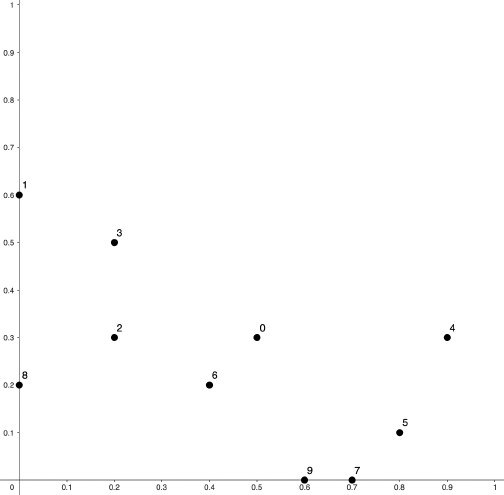
\includegraphics[width=0.35\linewidth]{images/skyline.png}
            \end{figure}
            We access the first row and since the window has no elements we add it to it. We check for every tuple if it dominates the inserted one. 
            Only the tuples three and one are not dominated by the tuple four, so the final window contains the points four, three and one. Graphically
            we have that the skyline of the given dataset is the following. 
            \begin{figure}[H]
                \centering
                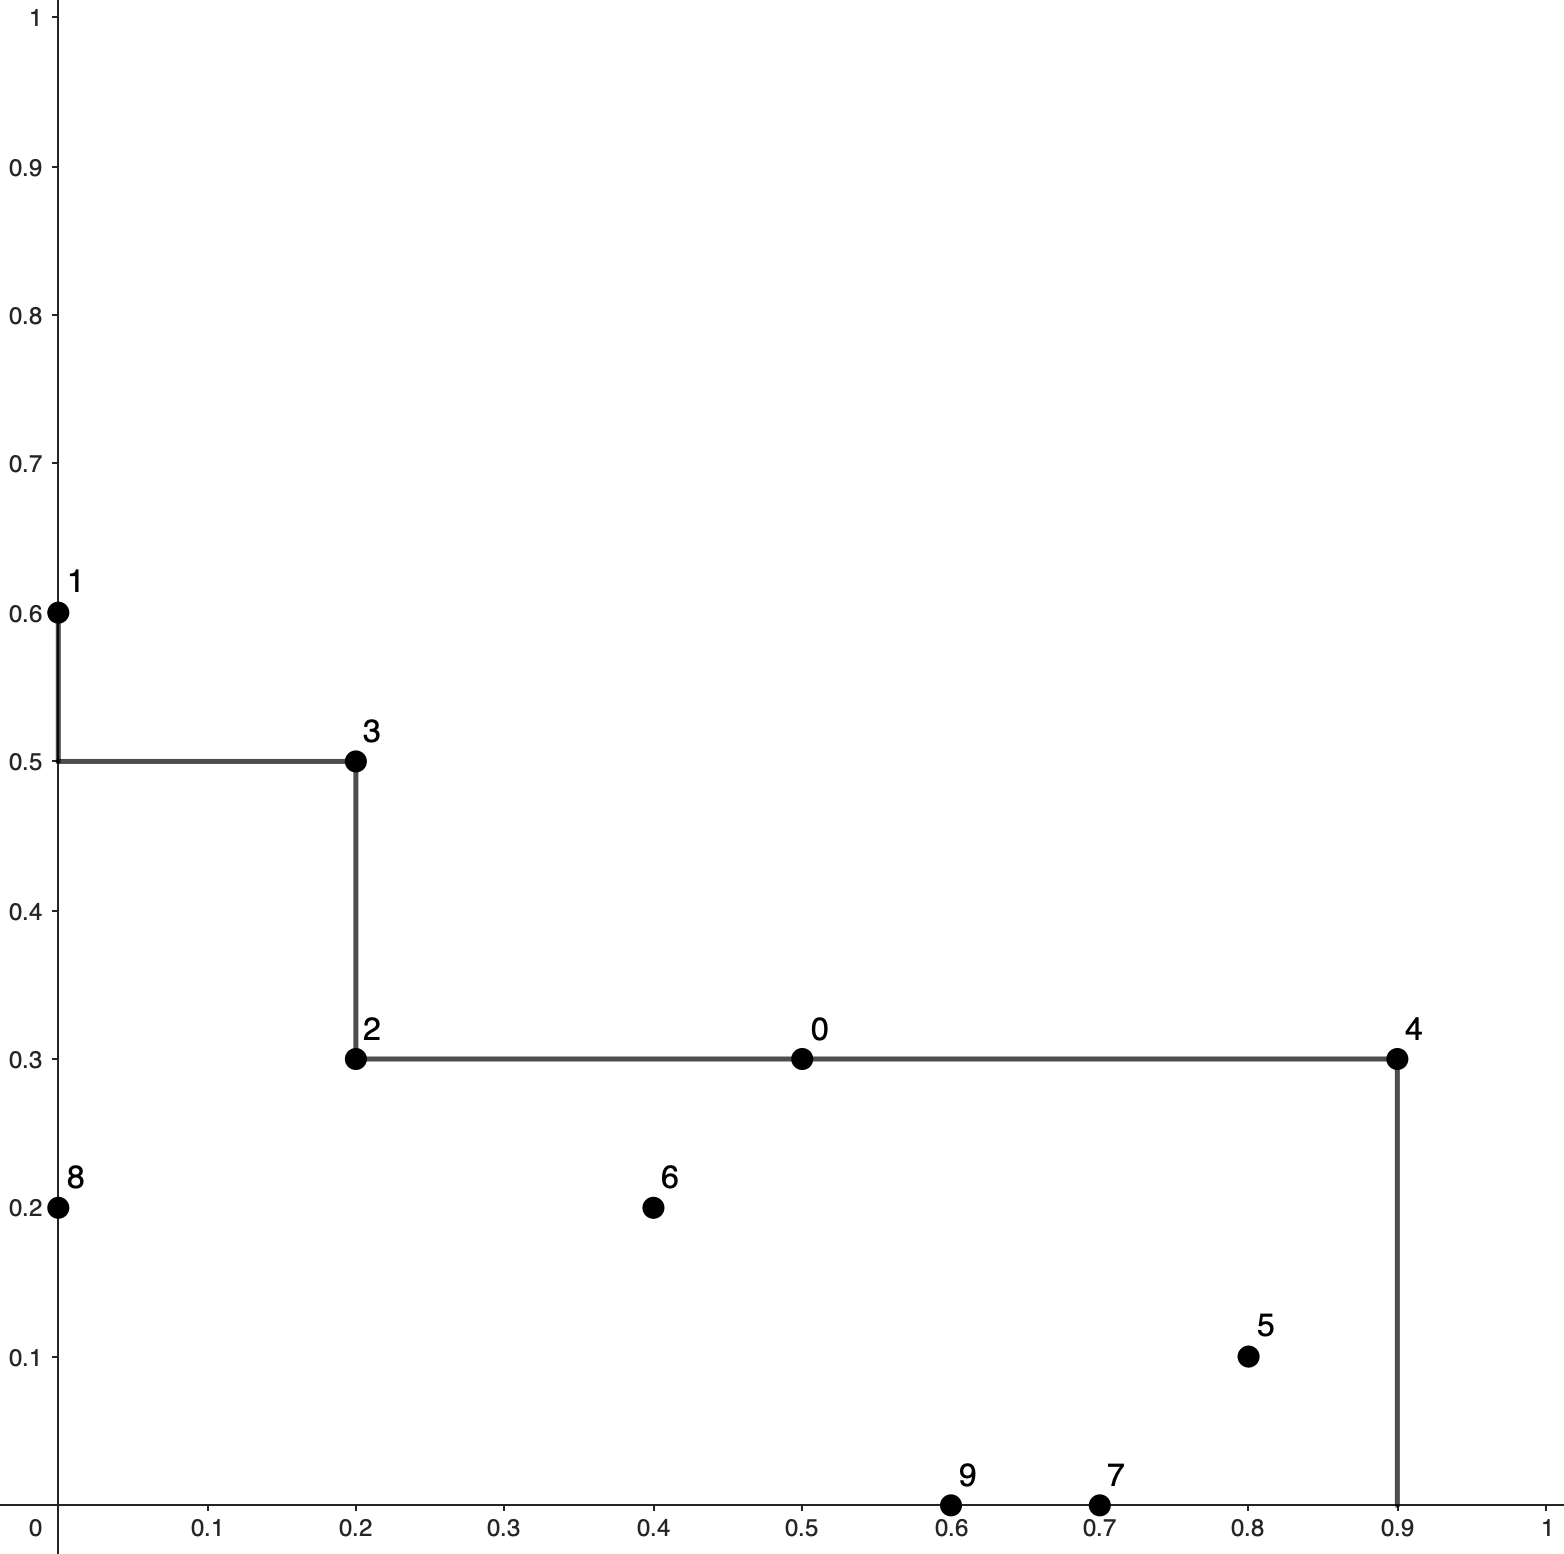
\includegraphics[width=0.35\linewidth]{images/skylinesol.png}
            \end{figure}
        \item Players zero and five are dominated only by player four, so they are part of the 2-skyband. Players one, three and four
            are part of the skyline, so they are obviously also part of the 2-skyband. 
            The 3-skyband is made of the players one, three, four, six and seven according to the definition. 
    \end{enumerate}

    \newpage 
    \section{Ranking and skyline queries}
        Consider the following three ranked lists reporting statistics about European soccer teams: 
        \begin{table}[H]
            \centering
            \begin{tabular}{|cc|cc|cc|}
            \hline
            \textbf{Goals} & \textbf{Team} & \textbf{Possession} & \textbf{Team} & \textbf{Passes} & \textbf{Team} \\ \hline
            75         & PSG      & 63.2         & BMU      & 89.9         & PSG      \\
            73         & BMU      & 62.1         & BAR      & 88.9         & MCY      \\
            70         & ATA      & 61.8         & PSG      & 88.4         & BAR      \\
            68         & MCY      & 61.6         & MCY      & 87.5         & BMU      \\
            68         & BDO      & 59.0         & LIV      & 86.6         & BDO      \\
            66         & LIV      & 58.5         & BDO      & 84.4         & LAZ      \\
            63         & BAR      & 55.7         & ATA      & 83.9         & LIV      \\
            60         & LAZ      & 50.1         & LAZ      & 83.4         & ATA      \\ \hline
            \end{tabular}
        \end{table}
        \begin{enumerate}
            \item Apply an algorithm that does not use random access to determine the best team according to the scoring function:
                \[S(\textnormal{team})=\max\{\textnormal{team.Goals},\textnormal{team.Possession},\textnormal{team.Passes}\}\]
            \item On this dataset, could you do better than the previous algorithm, in terms of access cost, with an algorithm that also uses random access? 
            \item Apply now the TA to determine the best team according to the same scoring function as in one. 
            \item Apply now the TA to determine the best team according to the following scoring function:
                \[S(\textnormal{team}) = \textnormal{team.Goals} + \textnormal{team.Possession} + \textnormal{team.Passes}\]
            \item Determine the skyline of the dataset. 
        \end{enumerate}
    \subsection*{Solution}
        \begin{enumerate}
            \item Since the scoring function is MAX we can use the $B_0$ algorithm. Find the best team means that we have $k=1$, so we 
                need to make only one sorted access. By accessing the first row we obtain the following buffer. 
                \begin{table}[H]
                    \centering
                    \begin{tabular}{c|ccc|c}
                    \hline
                    \textbf{Player} & \textbf{Goals} & \textbf{Possession} & \textbf{Passes} & \textbf{Score} \\ \hline
                    PSG             & 75             & ?                   & 89.9            & 89.9           \\
                    BMU             & ?              & 63.2                & ?               & 0.8            \\ \hline
                    \end{tabular}
                \end{table}
                The maximum score is given to PSG, that is the best team according to the MAX scoring function. 
            \item No algorithm could do better than reading at least the top scores on each list. 
            \item We have again $k=1$. We make a sorted access to the first row to compute the threshold value and 
                the objects to insert in the buffer. 
                \begin{table}[H]
                    \centering
                    \begin{tabular}{c|ccc|c}
                    \hline
                    \textbf{Player} & \textbf{Goals} & \textbf{Possession} & \textbf{Passes} & \textbf{Score} \\ \hline
                    PSG             & 75             & ?                   & 89.9            & 89.9           \\
                    BMU             & ?              & 63.2                & ?               & 0.8            \\ \hline
                    \end{tabular}
                \end{table}
                The threshold point has a value that is the MAX of the scores in the first row, that is $89.9$. We now make random 
                accesses to complete the data in the buffer (remember that the algorithm searches the missing data when it inserts a 
                new object in the buffer). 
                \begin{table}[H]
                    \centering
                    \begin{tabular}{c|ccc|c}
                    \hline
                    \textbf{Player} & \textbf{Goals} & \textbf{Possession} & \textbf{Passes} & \textbf{Score} \\ \hline
                    PSG             & 75             & 61.8                & 89.9            & 89.9           \\ \hline
                    \end{tabular}
                \end{table}
                Note that the passes for PSG are accessed before via random access, and later via sorted access. So at each iteration (except for 
                the third column) the algorithm makes a sorted access and two random accesses. Since the threshold has the same value as the score 
                of PSG, the algorithm halts and returns PSG as the best team. 
            \item We have to apply again TA with $k=1$, but with a different scoring function, so the result may change. The check for the 
                first row is the same as the previous point, except for the score.
                \begin{table}[H]
                    \centering
                    \begin{tabular}{c|ccc|c}
                    \hline
                    \textbf{Player} & \textbf{Goals} & \textbf{Possession} & \textbf{Passes} & \textbf{Score} \\ \hline
                    PSG             & 75             & 61.8                & 89.9            & 226.7           \\ \hline
                    \end{tabular}
                \end{table}
                The threshold is the sum of the values in the first row $228.1$. The threshold is greater than PSG score, so we need to make another 
                iteration. In the next row we find: BMU (223.7), BAR (213.5), and MCY (218.5). All these scores are lower than PSG one, so the buffer 
                remains the same. The threshold point has a value of $224$, that is less than PSG score, so the algorithm halts. The best team with 
                SUM is again PSG. 
            \item It is possible to represent the dataset in a graph with coordinates (Goals, Possession, Passes). By inspecting the ordered table we 
                add PSG to the window and all the other teams that are not dominated by it. The only teams not dominated by PSG are BMU and BAR. We have 
                found that the skyline of the dataset is composed by three teams: PSG, BMU, and BAR. 
        \end{enumerate}

    \newpage 

    \section{Ranking and skyline queries}
        Consider the following two ranked lists of hotels: 
        \begin{table}[H]
            \centering
            \begin{tabular}{cc|cc}
            \hline
            \textbf{Rating} & \textbf{Hotel} & \textbf{Stars} & \textbf{Hotels} \\ \hline
            0.8             & C              & 0.8            & F               \\
            0.4             & G              & 0.6            & E               \\
            0.4             & F              & 0.5            & G               \\
            0.3             & D              & 0.4            & A               \\
            0.3             & A              & 0.2            & D               \\
            0.2             & E              & 0.2            & C               \\
            0.1             & B              & 0.2            & B               \\ \hline
            \end{tabular}
        \end{table}
        \begin{enumerate}
            \item Apply FA and TA to determine the top hotel according to the scoring function: 
                \[\textnormal{MAX}(o) = \max\{\textnormal{Rating}(o), \textnormal{Stars}(o)\}\] 
            \item Indicate the number of sorted accesses and random accesses executed on each source. 
            \item Could FA make fewer sorted accesses than TA?
            \item Could FA make fewer random accesses than TA?
            \item TA is instance optimal: can any algorithm cost overall less than TA?
        \end{enumerate}
    \subsection*{Solution}
        \begin{enumerate}
            \item For the FA we have to make sorted access until we found $k$ objects in all tables. 
                In this case we need to find only one element that is in both columns. To do so we need 
                three sorted accesses, and we obtain the following buffer. 
                \begin{table}[H]
                    \centering
                    \begin{tabular}{c|cc|c}
                    \hline
                    \textbf{Hotel} & \textbf{Rating} & \textbf{Stars} & \textbf{Score} \\ \hline
                    F     & 0.4    & 0.8   & 1.2   \\
                    C     & 0.8    & ?     & 0.8   \\
                    G     & 0.4    & 0.5   & 0.9   \\
                    E     & ?      & 0.6   & 0.6   \\ \hline
                    \end{tabular}
                \end{table}
                We need to find the missing values with two random accesses, and we have
                \begin{table}[H]
                    \centering
                    \begin{tabular}{c|cc|c}
                    \hline
                    \textbf{Hotel} & \textbf{Rating} & \textbf{Stars} & \textbf{Score} \\ \hline
                    F     & 0.4    & 0.8   & 1.2   \\
                    C     & 0.8    & 0.2   & 1.0   \\
                    G     & 0.4    & 0.5   & 0.9   \\
                    E     & 0.2    & 0.6   & 0.8   \\ \hline
                    \end{tabular}
                \end{table}
                The best hotel according to the given scoring function is F. 

                The TA checks rows until the value of the threshold is greater than the worst score in the top-$k$. After accessing the first row 
                we have:
                \begin{table}[H]
                    \centering
                    \begin{tabular}{c|cc|c}
                    \hline
                    \textbf{Hotel} & \textbf{Rating} & \textbf{Stars} & \textbf{Score} \\ \hline
                    F     & 0.4    & 0.8   & 1.2   \\ \hline
                    \end{tabular}
                \end{table}
                With a threshold of $1.6$. After accessing the second row we have the same buffer, and a threshold value of $1.0$, that is less than F's score, so 
                the algorithm halts. The best hotel found is again F. 
            \item With FA we have made six sorted accesses (three for Rating, and three for Stars) and two random accesses (one for Rating, and one for Stars), so the total is eight. 
                With TA we have made four sorted accesses (two for Rating, and two for Stars) and four random accesses (two for Rating, and two for Stars), so the total is eight. 
            \item No, because FA stops its sorted access phase when all potential top-$k$ objects (according to any possible scoring function) have been seen, so at least $k$ objects 
                are no worse than the threshold according to any scoring function. 
            \item Yes, in this exercise we have an example. 
            \item Yes, it is possible. 
        \end{enumerate}
    
    \newpage 

    \section{Ranking and skyline queries}
        Consider the following lists reporting statistics about soccer players.
        \begin{table}[H]
            \centering
            \begin{tabular}{cc|cc}
            \hline
            \textbf{Goals} & \textbf{Player} & \textbf{Assists} & \textbf{Player} \\ \hline
            25             & LEW             & 17               & DEB             \\
            21             & RON             & 15               & SAN             \\
            19             & MES             & 12               & MES             \\
            18             & MBA             & 6                & NEY             \\
            15             & ILI             & 5                & MBA             \\
            14             & SAN             & 5                & ILI             \\
            13             & NEY             & 3                & RON             \\
            8              & DEB             & 3                & LEW             \\ \hline
            \end{tabular}
        \end{table}
        \begin{enumerate}
            \item Apply the TA to determine the top-$2$ players according to the scoring function: 
                \[S(\textnormal{player})=\textnormal{player.Goals}+\textnormal{player.Assists}\]
            \item Reuse as much as possible the answer of the previous question to indicate the 
                reached depth and the number of sorted and random accesses to determine, with TA,
                the top-$1$ player according to the same scoring function as the previous point.
            \item Discuss whether any algorithm could attain a lower execution cost than the cost 
                incurred by TA to determine the top-$1$ player. 
            \item Apply now the TA to determine the top-$2$ players according to the scoring function: 
                \[S(\textnormal{player})=\left\lvert \textnormal{player.Goals}-\textnormal{player.Assists} \right\rvert\]
            \item Determine the skyline of the dataset. 
        \end{enumerate}
    \subsection*{Solution}
        \begin{enumerate}
            \item The execution of the TA algorithm needs four rounds to stop on the given dataset. At the fourth 
                round we have the following buffer. 
                \begin{table}[H]
                    \centering
                    \begin{tabular}{c|cc|c}
                    \hline
                    \textbf{Player} & \textbf{Goals} & \textbf{Assists} & \textbf{Score} \\ \hline
                    MES             & 19             & 12               & 31             \\
                    SAN             & 14             & 15               & 29             \\ \hline
                    \end{tabular}
                \end{table}
                With a threshold value of $24$. We found that the best two players for the given scoring function
                are MES and SAN. 
            \item The procedure is the same as the previous point, but it stops at the third round since the threshold 
                condition is already verified at this step. The buffer is the following.
                \begin{table}[H]
                    \centering
                    \begin{tabular}{c|cc|c}
                    \hline
                    \textbf{Player} & \textbf{Goals} & \textbf{Assists} & \textbf{Score} \\ \hline
                    MES             & 19             & 12               & 31             \\ \hline
                    \end{tabular}
                \end{table}
                With a threshold of $31$. We have found that the best player is MES. 
            \item FA would stop at depth three as well, but only needs four random accesses to find the top player. 
            \item The given function is not monotone, so the TA can return wrong results. In this case the algorithm 
                will fail, returning DEB instead of RON. 
            \item After sorting the dataset we insert MES in the window. The only players that are not dominated by him
                are: SAN, LEW, and DEB. So, we have that the skyline is composed by these three players. 
        \end{enumerate}

    \chapter{Exercise session V}
        \section{Java Persistence API}
            An application lets an employee edit the projects he is responsible for. A project has a name, a start and end date and a budget. The employee can create 
            projects and assign other employees to them. Employees have a name, a code. Employees also have one or more skills. After logging in, the employee accesses 
            a home page that displays:
            \begin{itemize}
                \item The list of his projects, ordered by end date descending and with the list of employees allocated to each one. 
                \item The list of other employees, with the last name and the list of skills possessed. 
                \item A form for creating a project. 
                \item A form for choosing a project and assigning it to another employee. After creating a project or an assignment, the home page is displayed again, 
                    with the information updated. 
            \end{itemize}
            The entity relationship model is the following:
            \begin{figure}[H]
                \centering
                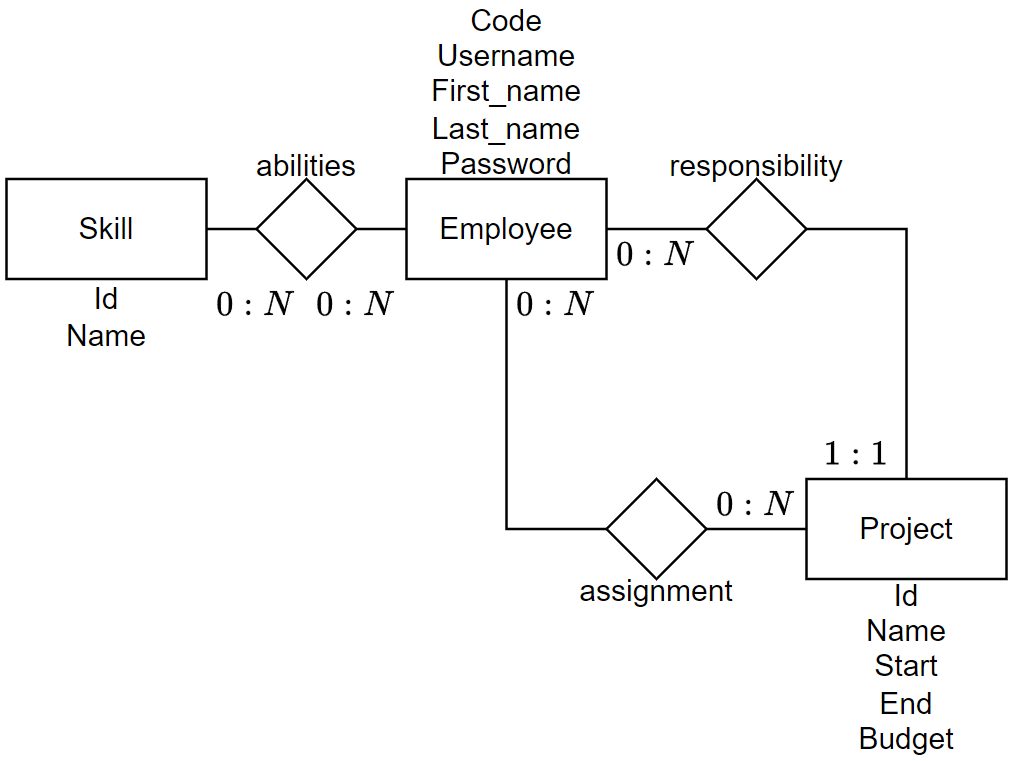
\includegraphics[width=0.5\linewidth]{images/e-r.png}
            \end{figure}
            The relational model is: 
            \begin{itemize}
                \item Project(\underline{id}, name, start, end, budget, responsible)
                \item Emp$\_$prj(\underline{empid}, \underline{prjid})
                \item Employee(\underline{code}, firstname, lastname, username, pwd)
                \item Skill$\_$emp(\underline{skillid}, \underline{empid})
                \item Skill(\underline{id}, label)
            \end{itemize}
            Given the specifications write the entity classes of the ORM mapping, including annotations for the attributes and for the relationships, fetch type of attributes
            and of relationships, and operation cascading policies for relationships (when not by default). 
        \subsection*{Solution}
            We start by checking all the relationships in the E-R diagram: 
            \begin{itemize}
                \item Responsibility: from employee to project we have to use the annotations: 
                    \begin{lstlisting}[style=Java]
@OneToMany
@OrderBy("end DESC")
                    \end{lstlisting}
                    From project to employee we have to use these annotations: 
                    \begin{lstlisting}[style=Java]
// This annotation can be omitted since it is implicit
@ManyToOne
                    \end{lstlisting}
                    The owner of the relation is entity project. 
                \item Assignment: from project to employee we have to use the annotations: 
                    \begin{lstlisting}[style=Java]
@ManyToMany
// To let the client access the employees working in a project via relationship navigation
FetchType.EAGER
                    \end{lstlisting}
                    From employee to project we have to use these annotations: 
                    \begin{lstlisting}[style=Java]
// This annotation can be omitted since it is implicit
@ManyToMany
                    \end{lstlisting}
                    The owner of the relation can be either project or employee. 
                \item Abilities: from employee to skill we have to use the annotations: 
                    \begin{lstlisting}[style=Java]
@ManyToMany
                    \end{lstlisting}
                    From skill to employee we have to use these annotations: 
                    \begin{lstlisting}[style=Java]
// This annotation can be omitted since it is implicit
@ManyToMany
                    \end{lstlisting}
                    The owner of the relation can be either skill or employee. 
            \end{itemize}
            We can now define the three entity mappings. The entity employee is defined as:  
            \begin{lstlisting}[style=Java]
@Entity
@NamedQueries({
    @NamedQuery(name = "Employee.findAllButOne", query ="SELECT e FROM Employee e WHERE e.code <> :empid"),...})
public class Employee implements Serializable {
    ...
    @Id
    @GeneratedValue(strategy = GenerationType.IDENTITY)
    private int code;

    private String firstname;
    private String lastname;
    private String password;
    private String username;

    @ManyToMany(mappedBy = "employees", fetch = FetchType.EAGER)
    private List<Project> assignedProjects;

    @OneToMany(mappedBy = "manager", fetch = FeatchType.EAGER)
    @OrderBy("end DESC")
    private List<Project> managedProjects;

    @ManyToMany(mappedBy = "employees", fetch = FetchType.EAGER)
    private List<Skill> skills;
    ...
}
            \end{lstlisting}
            The entity project is defined as:  
            \begin{lstlisting}[style=Java]
@Entity
@NamedQuery(name="Project.findAll",query="SELECT p FROM Project p")
public class Project implements Serializable {
    ...
    @Id
    @GeneratedValue(strategy=GenerationType.IDENTITY)
    private int id;

    private String name;
    private int budget;

    @Temporal(TemporalType.DATE)
    private Date start;

    @Temporal(TemporalType.DATE)
    private Date end;

    @ManyToMany(fetch = FetchType.EAGER)
    @JoinTable(name="emp_prj",
               joinColumns={@JoinColumn(name="projid")}, 
               inverseJoinColumns={@JoinColumn(name="empid")}
               )
    private List<Employee> employees;

    @ManyToOne
    @JoinColumn(name="responsible")
    private Employee manager;
    ...
}
            \end{lstlisting}
            The entity skill is defined as:  
            \begin{lstlisting}[style=Java]
@Entity
public class Skill implements Serializable {
    ...
    private static final long serialVersionUID = 1L;
    @Id
    @GeneratedValue(strategy=GenerationType.IDENTITY)
    private int id;
    private String label;
    @ManyToMany
    @JoinTable(name="skill_emp",
               joinColumns={@JoinColumn(name="skillid")},
               inverseJoinColumns={@JoinColumn(name="empid")}
               )
    private List<Employee> employees;
    ... 
}
            \end{lstlisting}
    \newpage 

    \section{Java Persistence API}
        An application permits the management of the bill of materials (BoM) of products. The BoM is the hierarchical description of a product in terms of the 
        sub-products that comprise it. At each level but the last one, a product is associated with the components that make it, each with a quantity. The application 
        allows the user to create BoMs. A BoM is progressively assembled by attaching to a product its sub-products and specifying the number of units of sub-products 
        that make one unit of the parent product. The editor accesses the HOME PAGE with the list of current BoMs and where s/he can create a new top level product and 
        view the existing BOMs. The editor can add product-sub-products links to a product, modify the quantity of a product-sub-products link, delete a product or
        product-sub-products link. Products have an identifier, a name a description and a unit cost. An example of BoM is the following: 
        \begin{figure}[H]
            \centering
            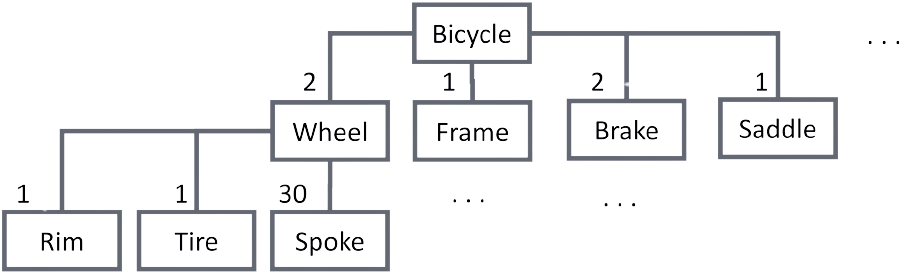
\includegraphics[width=0.6\linewidth]{images/BoM.png}
        \end{figure}
        The entity relationship model is the following:
        \begin{figure}[H]
            \centering
            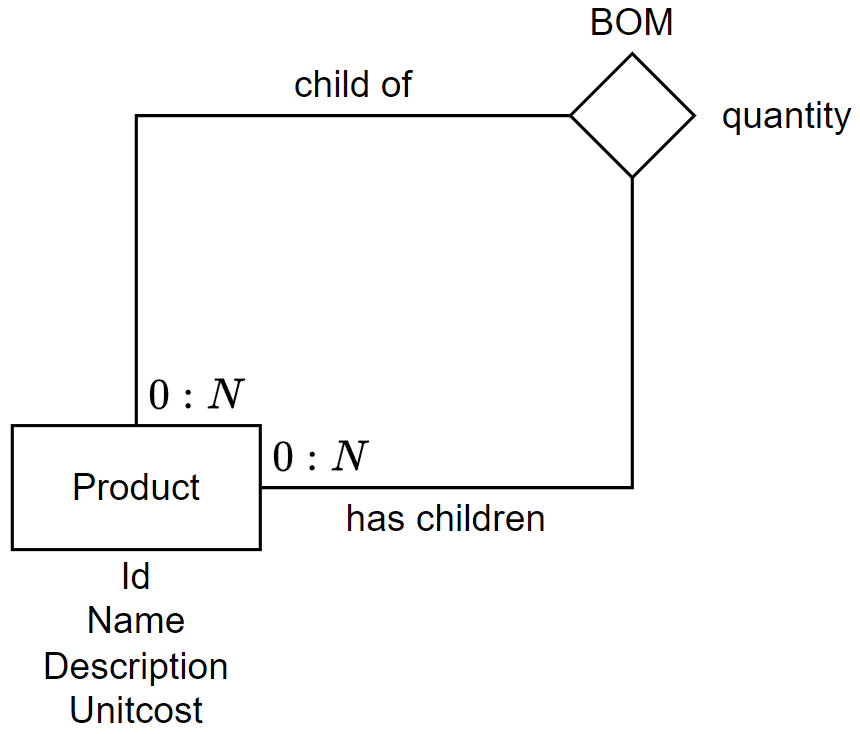
\includegraphics[width=0.3\linewidth]{images/e-r1.png}
        \end{figure}
        The relational schema DDL of the given database is: 
        \begin{lstlisting}[style=SQL]
CREATE TABLE 'product' (
    'id'            INT             NOT NULL AUTO_INCREMENT,
    'unitcost'      INT             NOT NULL,
    'name'          VARCHAR(45)     NOT NULL,
    'description'   VARCHAR(45)     DEFAULT NULL,
    PRIMARY KEY ('id')
) 
CREATE TABLE 'subparts' (
    'father'        INT             NOT NULL,
    'child'         INT             NOT NULL,
    'quantity'      INT             NOT NULL,
    PRIMARY KEY ('father','child'),
    KEY 'childtoproduct_idx' ('child'),
    CONSTRAINT 'childtoproduct' FOREIGN KEY ('child') REFERENCES 'product' ('id'),
    CONSTRAINT 'fathertoproduct' FOREIGN KEY ('father') REFERENCES 'product' ('id')
)           
        \end{lstlisting}
        The relational model is: 
        \begin{itemize}
            \item Product(\underline{id}, unitcost, name, description)
            \item Subparts(\underline{father}, \underline{child}, quantity)
        \end{itemize}
        Given the specifications, write the entity classes of the ORM mapping, including annotations for the attributes and for the relationships, fetch type of 
        attributes and of relationships, and operation cascading policies for relationships (when not by default).
    \subsection*{Solution}
        Given the specifications write the entity classes of the ORM mapping, including annotations for the attributes and for the relationships, fetch type of attributes
        and of relationships, and operation cascading policies for relationships (when not by default). 

        \begin{itemize}
            \item BoM: from father product to children product we have to use the annotations: 
                \begin{lstlisting}[style=Java]
@ManyToMany
                \end{lstlisting}
                From children product to father product we have to use these annotations: 
                \begin{lstlisting}[style=Java]
@ManyToMany
                \end{lstlisting}
                The owner of the relation is entity project. 
            \item 
        \end{itemize}
        The entity product is defined as:  
            \begin{lstlisting}[style=Java]
@Entity
@NamedQueries({
@NamedQuery(name = "BomProduct.findAll", query = "SELECT p FROM BomProduct p"),
@NamedQuery(name = "BomProduct.findAllTop", query = "SELECT p FROM BomProduct p WHERE p.fathers IS EMPTY") })

public class BomProduct implements Serializable {
    ...
    private static final long serialVersionUID = 1L;
    @Id @Column(name="id") @GeneratedValue(strategy = GenerationType.IDENTITY)
    private int id;
    private String description;
    private String name;
    private int unitcost;
    ...
    @ElementCollection(fetch = FetchType.EAGER)
    @CollectionTable(name = "subparts",joinColumns = @JoinColumn(name = "father"))
    @MapKeyJoinColumn(name = "child")
    @Column(name = "QUANTITY")
    private Map<BomProduct, Integer> subparts;
    
    @ManyToMany
    @JoinTable(name = "subparts",
               joinColumns = @JoinColumn(name = "child"),
               inverseJoinColumns = @JoinColumn(name ="father"))
    private List<BomProduct> fathers;
    ...            
}
            \end{lstlisting}
        The better way is to make the many-to-many relationships with attributes a weak entity like in the following image. 
        \begin{figure}[H]
            \centering
            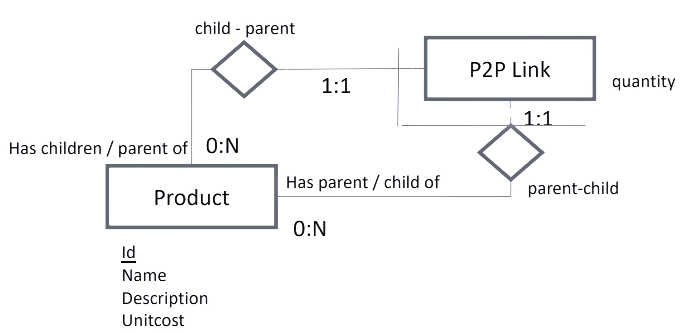
\includegraphics[width=0.6\linewidth]{images/BoMweak.png}
        \end{figure}
        The entity P2PLinkID is defined as:  
        \begin{lstlisting}[style=Java]
@Embeddable
public class P2PLinkID implements Serializable {
    private static final long serialVersionUID = 1L;
    private int father;
    private int child;

    public P2PLinkID() { }
    
    public P2PLinkID(int father, int child) {
        super();
        this.father = father;
        this.child = child;
    }
    ...
}
        \end{lstlisting}
        The entity P2PLink is defined as:  
        \begin{lstlisting}[style=Java]
@Entity
public class P2PLink implements Serializable {
    private static final long serialVersionUID = 1L;
    
    @EmbeddedId
    private P2PLinkID id;

    @ManyToOne
    @MapsId("father") // reference to the foreign key attribute
    @JoinColumn(name = "father")
    private BomProduct father;

    @ManyToOne
    @MapsId("child") // reference to the foreign key attribute
    @JoinColumn(name = "child")
    private BomProduct child;

    private int quantity;
    ...
}
        \end{lstlisting}
        The entity product is defined as:  
        \begin{lstlisting}[style=Java]
@Entity
public class BomProduct implements Serializable {
    private static final long serialVersionUID = 1L;

    @Id @GeneratedValue(strategy = GenerationType.IDENTITY)
    private int id;
    private String description;
    private String name;
    private int unitcost;

    // getters setters and constructors

    @OneToMany(mappedby="father")
    private List<P2PLink> children;

    @OneToMany(mappedby="child")
    private List<P2PLink> fathers;
    ...
}
        \end{lstlisting}




\end{document}